\documentclass[a4paper,11pt]{article}
\usepackage[verbose,a4paper,tmargin=2cm,bmargin=2cm,lmargin=2.5cm,rmargin=2.5cm]{geometry}
\usepackage{polski}
\usepackage{amsmath}
\usepackage{amsfonts}
\usepackage{amssymb}
\usepackage{lastpage}
\usepackage{indentfirst}
\usepackage{verbatim}
\usepackage{graphicx}
\usepackage{fancyhdr}
\usepackage{listings}
\usepackage{float}
\usepackage{hyperref}
\hypersetup{
    colorlinks = true,
    linkcolor = black,
    urlcolor = cyan
}
\usepackage{xcolor}
\usepackage{tikz}
\usepackage{multirow}
\frenchspacing
\pagestyle{fancyplain}
\fancyhf{}

\usepackage{setspace}
\usepackage{enumitem}

\renewcommand{\headrulewidth}{0pt}
\renewcommand{\footrulewidth}{0.4pt}
\newcommand{\degree}{\ensuremath{^{\circ}}} 
\fancyfoot[L]{MUM: P. Galewicz, B. Jurczewski, Z. Nowacki, K.Podlewski, P. Wardęcki}
\fancyfoot[R]{\thepage\ / \pageref{LastPage}}

\begin{document}

%%%%%%%%%%%%%%%%%%%%%%%%%%%%%%%%%%%%%%%%%%%% STRONA TYTUŁOWA

\begin{titlepage}
\begin{center}
\begin{tabular}{rcl}
\begin{tabular}{|r|}
\hline \\
\large{\underline{234053~~~~~~~~~~~~~~~~~~~~~~~} }\\
\small{\textit{Numer indeksu}}\\
\large{\underline{Paweł Galewicz~~~~~~~~~~~~} }\\
\small{\textit{Imię i nazwisko}}\\\\ \hline
\end{tabular} 
&
\begin{tabular}{|r|}
\hline \\
\large{\underline{234067~~~~~~~~~~~~~~~~~~~~~~~} }\\
\small{\textit{Numer indeksu}}\\
\large{\underline{Bartosz Jurczewski~~~~~~~} }\\
\small{\textit{Imię i nazwisko}}\\\\ \hline
\end{tabular} 
&
\begin{tabular}{|r|}
\hline \\
\large{\underline{234102~~~~~~~~~~~~~~~~~~~~~~~} }\\
\small{\textit{Numer indeksu}}\\
\large{\underline{Zbigniew Nowacki~~~~~~~~} }\\
\small{\textit{Imię i nazwisko}}\\\\ \hline
\end{tabular} 
\end{tabular} 

\vspace{10px}

\begin{tabular}{rl}
\begin{tabular}{|r|}
\hline \\
\large{\underline{234106~~~~~~~~~~~~~~~~~~~~~~~} }\\
\small{\textit{Numer indeksu}}\\
\large{\underline{Karol Podlewski~~~~~~~~~~~} }\\
\small{\textit{Imię i nazwisko}}\\\\ \hline
\end{tabular} 
&
\begin{tabular}{|r|}
\hline \\
\large{\underline{234128~~~~~~~~~~~~~~~~~~~~~~~} }\\
\small{\textit{Numer indeksu}}\\
\large{\underline{Piotr Wardęcki~~~~~~~~~~~~} }\\
\small{\textit{Imię i nazwisko}}\\\\ \hline
\end{tabular} 
\end{tabular}
\end{center}

\vspace{25px}

\begin{tabular}{ll}
\LARGE{\textbf{Kierunek}}& \LARGE{Informatyka Stosowana} \\
\LARGE{\textbf{Stopień}}& \LARGE{II} \\
\LARGE{\textbf{Specjalizacja}}& \LARGE{Data Science} \\
\LARGE{\textbf{Semestr}}& \LARGE{1} \\\\
\LARGE{\textbf{Data oddania}}& \LARGE{15 kwietnia 2020} \\\\\\\\\\\\\\
\end{tabular}

\begin{center}
\textbf{\huge{\\~\\Metody uczenia maszynowego }}
\textbf{\Huge{\\~\\Problem set 2}}
\end{center}

\end{titlepage}

\setcounter{page}{2}
\setstretch{1.5}
\tableofcontents
\newpage
\setstretch{1.1}

%%%%%%%%%%%%%%%%%%%%%%%%%%%%%%%%%%%%%%%%%%%% CEL

\section{Cel} \label{sec:cel}
Zadanie polegało na analizie procesu grupowania danych za pomocą wybranych metod:

\begin{enumerate}
    \item Algorytmu EM,
    \item Algorytmu k-średnich,
    \item Algorytmu hierarchiczne aglomeracyjnego,
    \item Metody gęstościowej DBSCAN,
    \item metoda optics.
\end{enumerate}

Należało zaimplementować każdą metodę, a następnie zweryfikować jej działanie biorąc pod uwagę:

\begin{itemize}
    \item Rożne możliwe ustawienia parametrów konfiguracyjnych i ich wpływ na wyniki klasyfikacji,
    \item Zbiory danych o różnej charakterystyce (przynajmniej 3 różne zbiory).
\end{itemize}

Każdą metodę należało przetestować na tych samych zbiorach, a następnie porównać wyniki i wyciągnąć wnioski dotyczące skuteczności poszczególnych metod. Jako kryterium porównawcze wykorzystaliśmy metryki \textit{Silhouette}, \textit{Calinski-Harabasz} oraz \textit{Daves-Bouldin}.

%%%%%%%%%%%%%%%%%%%%%%%%%%%%%%%%%%%%%%%%%%%% OPIS IMPLEMENTACJI

\section{Opis implementacji}

Algorytmy zostały zaimplementowane za pomocą języka Python w wersji 3.8.2.
Wykorzystano w nim biblioteki NumPy, Sklearn i Pandas. 

%%%%%%%%%%%%%%%%%%%%%%%%%%%%%%%%%%%%%%%%%%%% OPIS ZBIORÓW DANYCH

\section{Opis zbiorów danych} \label{sec:dataset}

Bazowaliśmy na trzech zestawach danych:

\begin{enumerate}[label=\Alph*.] \label{enum:datasets}
    \item{\href{https://www.kaggle.com/vjchoudhary7/customer-segmentation-tutorial-in-python}{Mall Customer Segmentation}} - Zawiera informacje zbierane od klientów centrum handlowego uczestniczących w programie lojalnościowym. Są to między innymi dane o wieku, płci, rocznym przychodzie. Każdy klient ma też wyliczoną ocenę wydatków w sklepie w przedziale od 1 do 100.
    \item{\href{https://www.kaggle.com/maitree/wine-quality-selection#winequality-red.csv}{Wine quality selection}} -- Zestaw danych przedstawiający współczynniki wina wraz z przyporządkowaną ich jakością.
    \item{\href{https://www.kaggle.com/arjunbhasin2013/ccdata}{Credit Card Dataset}} -- Zbiór opisujący zachowania aktywnych klientów bankowych, agregowanych przez 6miesięcy.
\end{enumerate}

\section{Klasyfikatory}

\subsection{Algorytm EM}

Algorytm Oczekiwania-Maksymalizacji (ang. \textit{Expectation-Maximization}, EM) wylicza rozkłady prawdopodobieństwa przynależności obserwacji do skupień. Jego przebieg rozpoczyna się od podania liczby centrów. Dla każdego z nich losowana jest jedna obserwacja, która będzie reprezentowała dane skupienie. Następnie powtarzane są dwa kroki aż do osiągnięcia wymaganej zbieżności:

\begin{itemize}
    \item oczekiwanie -- liczenie prawdopodobieństwa przynależności obserwacji do skupień
    \item maksymalizacja -- wyznaczenie wartości parametrów skupień, przy których wiarygodność rozkładu jest maksymalna
\end{itemize}

Parametry, które postanowiono przetestować jest liczba maksymalnych iteracji algorytmu oraz typ macierzy kowariancji.

\subsection{Algorytm k-średnich}

Algorytm k-średnich dzieli zbiór przypadków na k skupień, gdzie k jest podaną wartością. Rozpoczynając działanie od losowo wybranych środków skupień, przypisuje do nich obiekty biorąc pod uwagę odległość obiektów od wybranych środków. Kiedy obiekty zostały przypisane, wyznaczane są nowe środki, które zostają wyliczone na podstawie wartości atrybutów obiektów należących do danej grupy skupień.

Algorytm wymaga wcześniejszego określenia liczby skupień oraz maksymalnej liczby iteracji, po której przestanie dalej przetwarzać dane jeżeli wcześniej nie osiągnął stabilizacji. W przypadku zaprezentowanego rozwiązania użytkownik ma też wpływ na początkowe rozłożenie centrów oraz ilość przeprowadzonych losowań centrów w obrębie jednego uruchomienia algorytmu. 

\subsection{Algorytm hierarchiczny aglomeracyjny}
Metody hierarchiczne aglomeracyjne na początku traktują wszystkie obserwacje jak osobne klastry. W kolejnych krokach najbardziej zbliżone do siebie pary klastrów są ze sobą łączone - poruszamy się w górę hierarchii.
Dostępne parametry to:
\begin{itemize}
    \item metryka
    \begin{itemize}
        \item euklidesowa $ d\left( p,q\right) = \sqrt {\sum _{i} \left( q_{i}-p_{i}\right)^2 } $
        \item manhattan $ d\left( p,q\right) = \sum _{i} \left| q_{i}-p_{i}\right| $
    \end{itemize}
    \item metoda łączenia
    \begin{itemize}
        \item Warda -- odległość między klastrami jest sumą kwadratów odchyleń od punktów do centroidów. Dąży do zminimalizowania sumy kwadratów wewnątrz klastra
        \item kompletne -- odgległość między klastrami jest maksymalną odległością między obserwacją w jednym i drugim klastrze. Wrażliwy na obserwacje odstające od pozostałych w próbie.
        \item średnie -- odległość między klastrami jest średnią odległością między obserwacjami w jednym i drugim klastrze
        \item pojedyncze -- odległość między klastrami jest minimalną odległością między obserwacjami w jednym i drugim klastrze. Najlepsze kiedy klastry są wyraźnie oddzielone 
    \end{itemize}
\end{itemize}

Parametry, które postanowiono przetestować to obie metryki oraz metody połączeń pojedynczych i średnich.

\subsection{Metoda gęstościowa DBSCAN}
Algorytm klasteryzcji opracowany pod koniec lat 90 ubiegłego wieku. Jego klasteryzacja opiera się na gęstości punktów w skupieniach. Przyjmując na wejściu zbiór punktów, grupuje razem te punkty które są najbliższymi sąsiadami (najbliżej "upakowane"). Należy do grona najpopularniejszych algorytmów i jest najczęściej wspominanym w naukowej literaturze. 

\subsection{Algorytm optics}
Algorytm ten jest algorytmem w oparciu o znalezienie gęstości klastrów w danych przestrzennych. Jest algorytmem zbliżonym do algorytmu DBSCAN jednak z pewnymi przewagami, potrafi wykrywać znaczące klastry w danych o różnej gęstości. W tym celu punkty danych są uporządkowane liniowo w taki sposób, że najbliższe przestrzennie punkty stają się sąsiadami. Dla każdego punktu zapisywana jest specjalna odległość reprezentująca gęstość oraz określająca przynależność do konkretnego zbioru.


%%%%%%%%%%%%%%%%%%%%%%%%%%%%%%%%%%%%%%%%%%%% BADANIA

\section{Badania}

W sekcji badań odnoszono się do zbiorów danych za pomocą oznaczeń zgodnych z sekcją \ref{sec:dataset}.

Przy badaniu wykorzystano następujące metryki:

\begin{enumerate}
    \item Indeks Silhouette,
    \item Indeks Calińskiego-Harabasza,
    \item Indeks Daviesa-Bouldina.
\end{enumerate}

Żadna z metryk nie odnosi się do oczekiwanych rezultatów. Dla każdej z nich lepszym wynikiem będzie wyższa liczba. Nie można jednak porównywać metryk między sobą.

Porównywanie uzyskanych rezultatów pomiędzy algorytmami także nie jest wysoce miarodajne - metryki mogą oczekiwać przypasowania danych w określony sposób, niezależnie od użytego algorytmu. Będzie to promować rozwiązania, które są bliżej oczekiwanego wzorca, nie zawsze będąc faktycznie optymalnym podziałem dla danego zbioru danych \cite{ClusteringQuality}. Dlatego zdecydowaliśmy się nie porównywać bezpośrednio uzyskanych wyników pomiędzy różnymi algorytmami.


\subsection{Liczba centrów dla zbiorów danych}

W celu odpowiedniego doboru liczby centrów dla algorytmów Oczekiwania-Maksymalizacji, k-średnich oraz hierarchicznie aglomeracyjnego przeprowadzano testy wykorzystując metodę "łokcia" (która wykorzystuje algorytm k-średnich).

\begin{figure}[H]
    	\centering
    	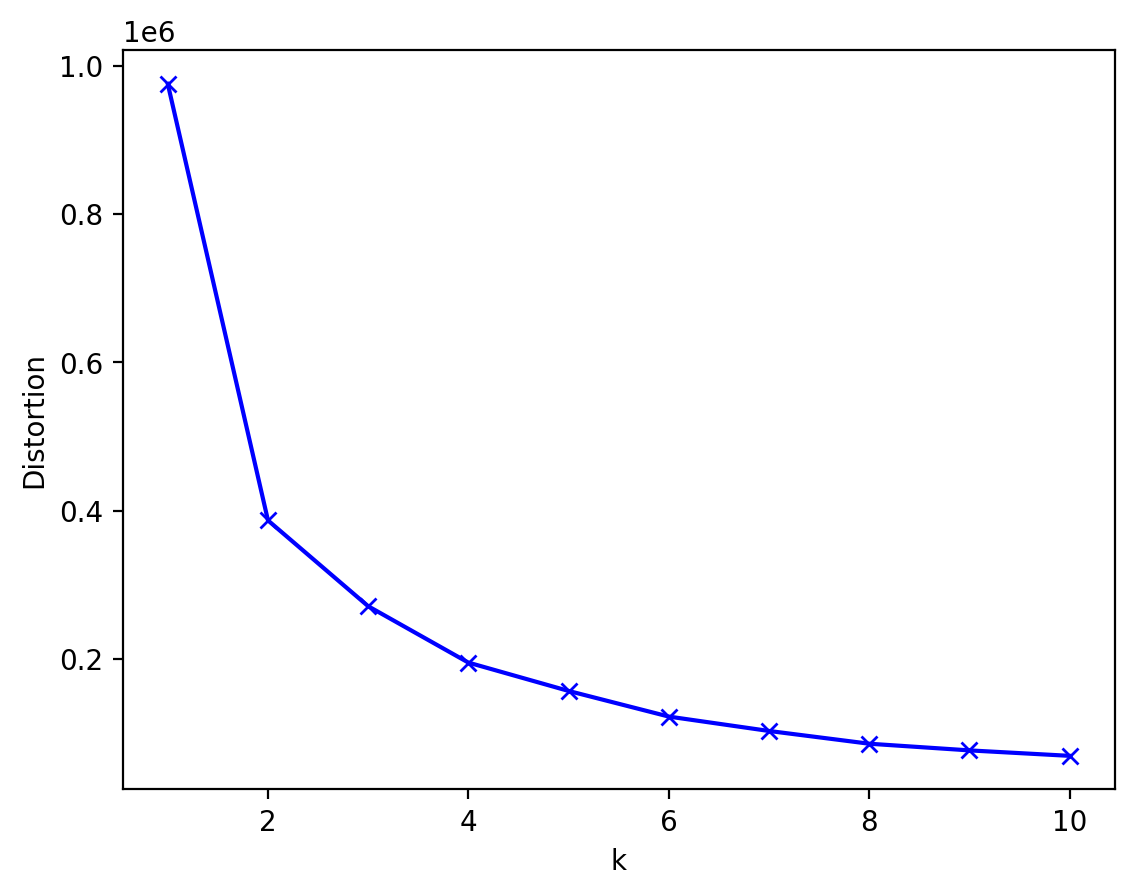
\includegraphics[width=0.67\textwidth]{images2/elbow_Customer.png}
    	\caption{Metoda "łokcia" dla zbioru danych A}
    	\label{fig:e1}
\end{figure}

\begin{figure}[H]
    	\centering
    	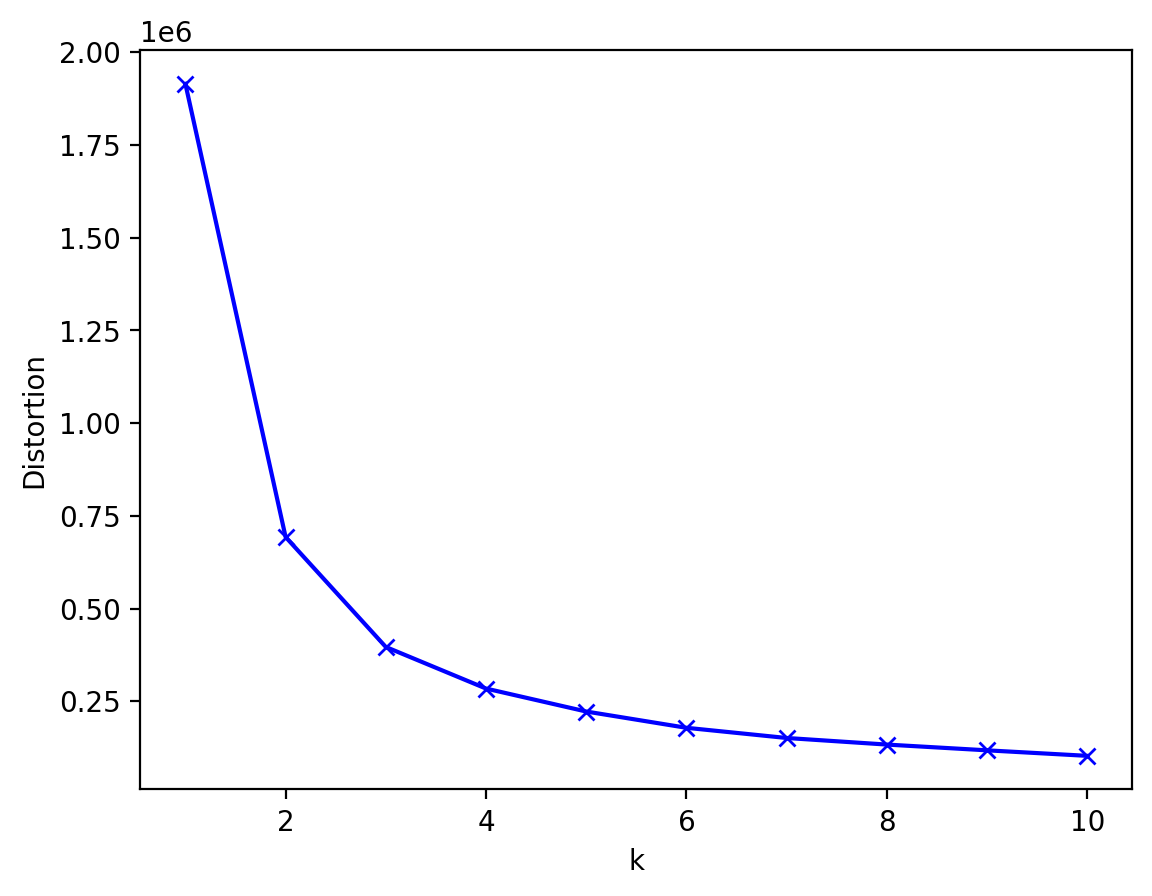
\includegraphics[width=0.67\textwidth]{images2/elbow_Wines.png}
    	\caption{Metoda "łokcia" dla zbioru danych B}
    	\label{fig:e2}
\end{figure}

\begin{figure}[H]
    	\centering
    	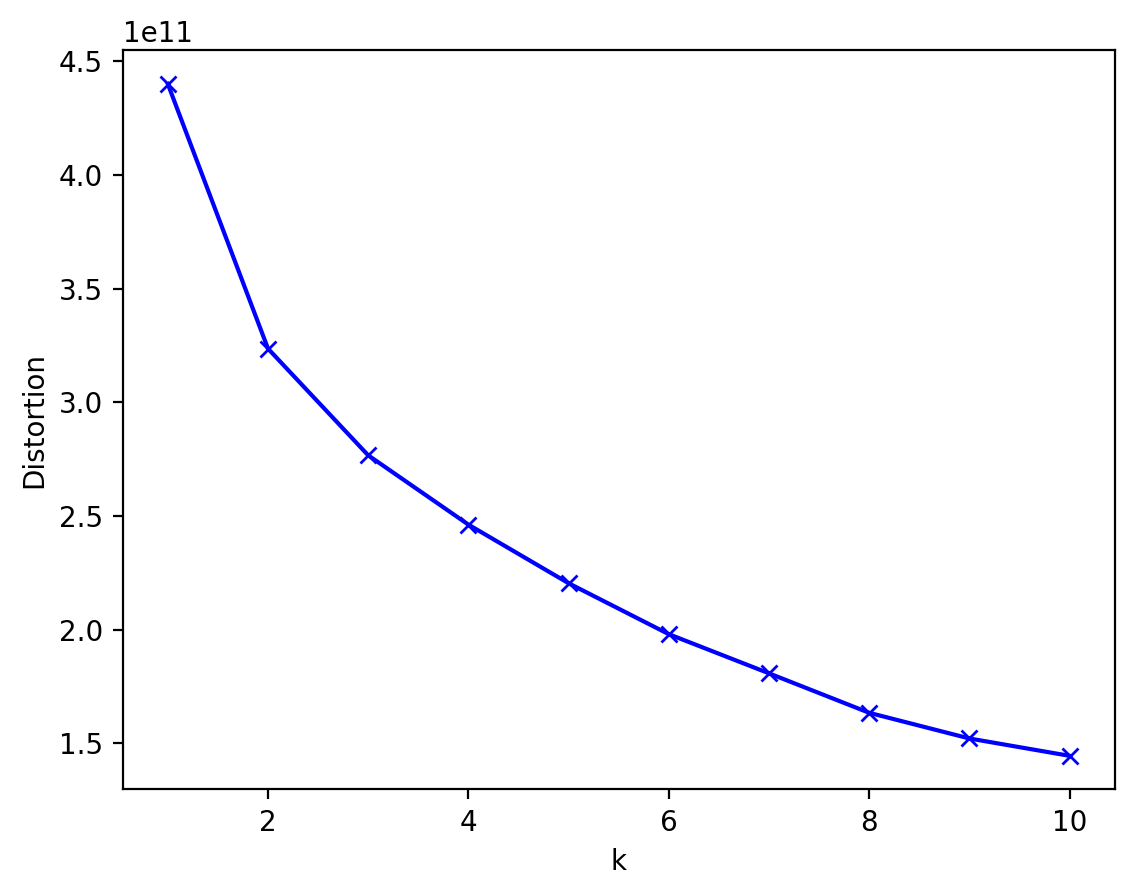
\includegraphics[width=0.67\textwidth]{images2/elbow_CC.png}
    	\caption{Metoda "łokcia" dla zbioru danych C}
    	\label{fig:e3}
\end{figure}

Wyniki uzyskane z wykorzystaniem metody "łokcia" dla zbioru danych A sugerowały użycie 4 lub 5 klastrów - my zdecydowaliśmy się na ten drugi wariant. W przypadku danych B były to 4 klastry, a w przypadku danych C - 3 klastry.

\subsection{Algorytm EM}

\subsubsection*{Zbiór A}

\begin{table}[H]
    \centering
    \begin{tabular}{|l|l|l|l|}
    \hline
    \textbf{Typ kowariancji} & \textbf{Silhouette} & \textbf{Calinski-Harabasz} & \textbf{Davies-Bouldin} \\ \hline
    full                     & 0.35                & 223.102                    & 0.905                   \\ \hline
    tied                     & 0.398               & 212.722                    & 0.898                   \\ \hline
    diag                     & 0.343               & 231.842                    & 0.989                   \\ \hline
    spherical                & 0.442               & 251.828                    & 0.79                    \\ \hline
    \end{tabular}
    \caption{Wartości metryk dla różnych typów macierzy kowariancji algorytmu EM dla zbioru A}
    \label{tab:em_a_cov}
\end{table}

\begin{table}[H]
    \centering
    \begin{tabular}{|l|l|l|l|}
    \hline
    \textbf{Iteracja} & \textbf{Silhouette} & \textbf{Calinski-Harabasz} & \textbf{Davies-Bouldin} \\ \hline
    20                & 0.379               & 229.571                    & 0.893                   \\ \hline
    40                & 0.351               & 214.546                    & 0.974                   \\ \hline
    60                & 0.379               & 229.571                    & 0.893                   \\ \hline
    80                & 0.351               & 214.546                    & 0.974                   \\ \hline
    100               & 0.444               & 243.475                    & 0.737                   \\ \hline
    120               & 0.313               & 163.594                    & 1.176                   \\ \hline
    140               & 0.397               & 211.897                    & 0.899                   \\ \hline
    160               & 0.407               & 247.42                     & 0.893                   \\ \hline
    180               & 0.33                & 197.16                     & 0.954                   \\ \hline
    200               & 0.351               & 214.546                    & 0.974                   \\ \hline
    \end{tabular}
    \caption{Wartości metryk dla różnej maksymalnej liczby iteracji algorytmu EM dla zbioru A}
    \label{tab:em_a_iter}
\end{table}

Na podstawie tabel \ref{tab:em_a_cov} oraz \ref{tab:em_a_iter} wywnioskowano, że najkorzystniejsze wyniki wychodzą dla typu kowariancji\textit{"full"} oraz maksymalnej liczbie iteracji na poziomie 160. Konfigurację tę wykorzystano do wizualizacji danych na rysunku \ref{fig:em_a_1}.

\begin{figure}[H]
    \centering
    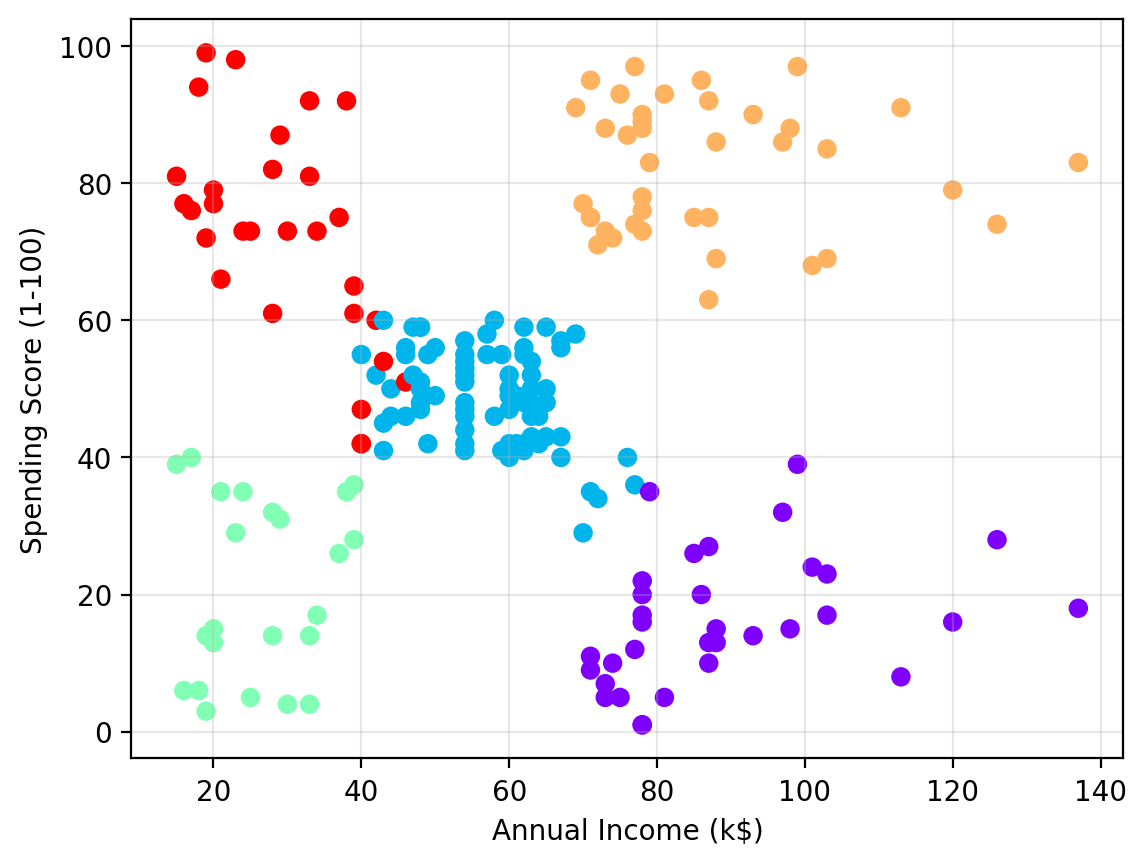
\includegraphics[width=0.67\textwidth]{images2/EM/mall/EM_Customer_xAnnualIncome_ySpendingScore.png}
    \caption{Wizualizacja wyliczonych centrów dla zbioru A przy pomocy EM}
    \label{fig:em_a_1}
\end{figure}

\subsubsection*{Zbiór B}

\begin{table}[H]
    \centering
    \begin{tabular}{|l|l|l|l|}
    \hline
    \textbf{Typ kowariancji} & \textbf{Silhouette} & \textbf{Calinski-Harabasz} & \textbf{Davies-Bouldin} \\ \hline
    full                     & -0.165              & 82.86                      & 4.17                    \\ \hline
    tied                     & 0.286               & 702.037                    & 1.273                   \\ \hline
    diag                     & -0.162              & 101.208                    & 6.883                   \\ \hline
    spherical                & 0.368               & 2116.932                   & 0.815                   \\ \hline
    \end{tabular}
    \caption{Wartości metryk dla różnych typów macierzy kowariancji algorytmu EM dla zbioru B}
    \label{tab:em_b_cov}
\end{table}

\begin{table}[H]
    \centering
    \begin{tabular}{|l|l|l|l|}
    \hline
    \textbf{Iteracja} & \textbf{Silhouette} & \textbf{Calinski-Harabasz} & \textbf{Davies-Bouldin} \\ \hline
    20                & 0.048               & 338.056                    & 3.437                   \\ \hline
    40                & -0.157              & 124.091                    & 7.692                   \\ \hline
    60                & -0.165              & 82.86                      & 4.17                    \\ \hline
    80                & -0.156              & 124.344                    & 7.692                   \\ \hline
    100               & -0.004              & 77.789                     & 10.078                  \\ \hline
    120               & -0.11               & 93.36                      & 5.182                   \\ \hline
    140               & -0.117              & 98.011                     & 6.9                     \\ \hline
    160               & -0.156              & 124.344                    & 7.692                   \\ \hline
    180               & -0.105              & 91.154                     & 5.671                   \\ \hline
    200               & -0.156              & 124.344                    & 7.692                   \\ \hline
    \end{tabular}
    \caption{Wartości metryk dla różnej maksymalnej liczby iteracji algorytmu EM dla zbioru B}
    \label{tab:em_b_iter}
\end{table}

Najlepszą konfiguracją dla zbioru B jest \textit{tied} oraz 100 iteracji. Na jej podstawie wygenerowano wykresy.

\begin{figure}[H]
    \centering
    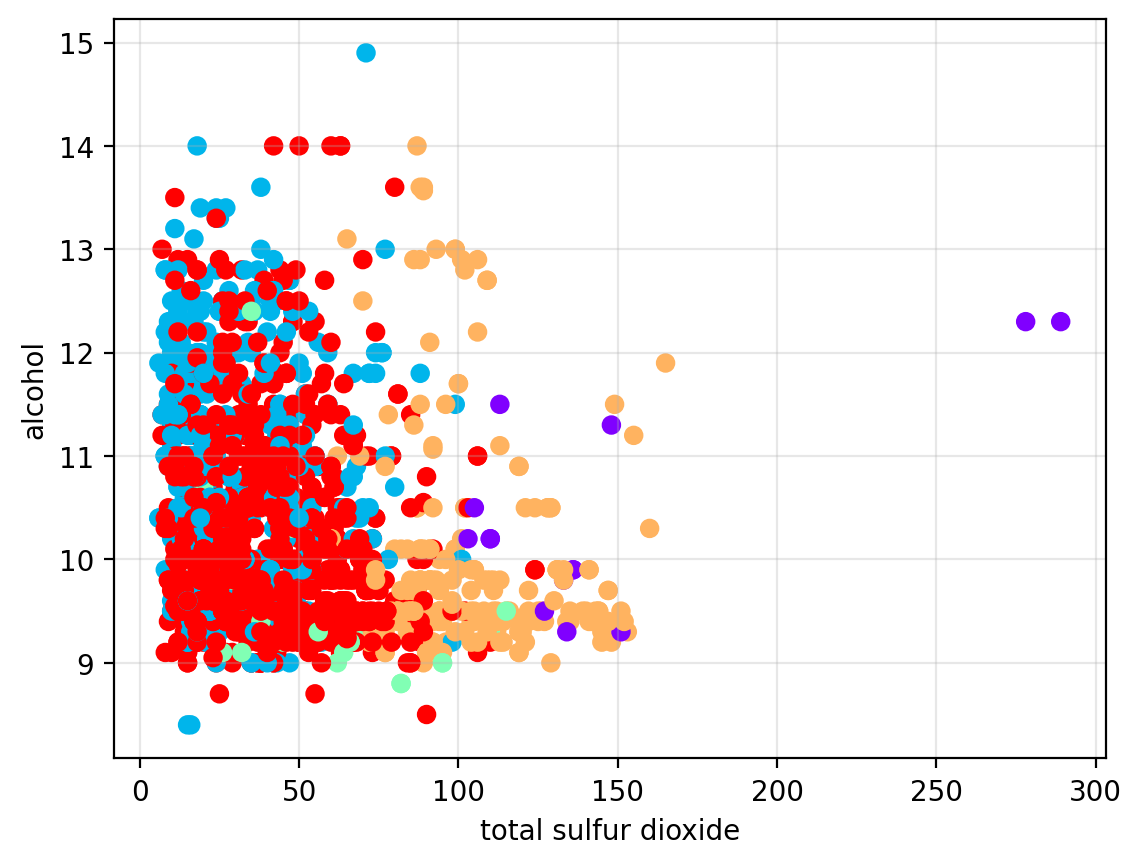
\includegraphics[width=0.67\textwidth]{images2/EM/wines/ExpectationMaximization_Wines_xtotalsulfurdioxide_yalcohol.png}
    \caption{Wizualizacja centrów dla zbioru B przy pomocy EM}
    \label{fig:em_b_1}
\end{figure}

\begin{figure}[H]
    \centering
    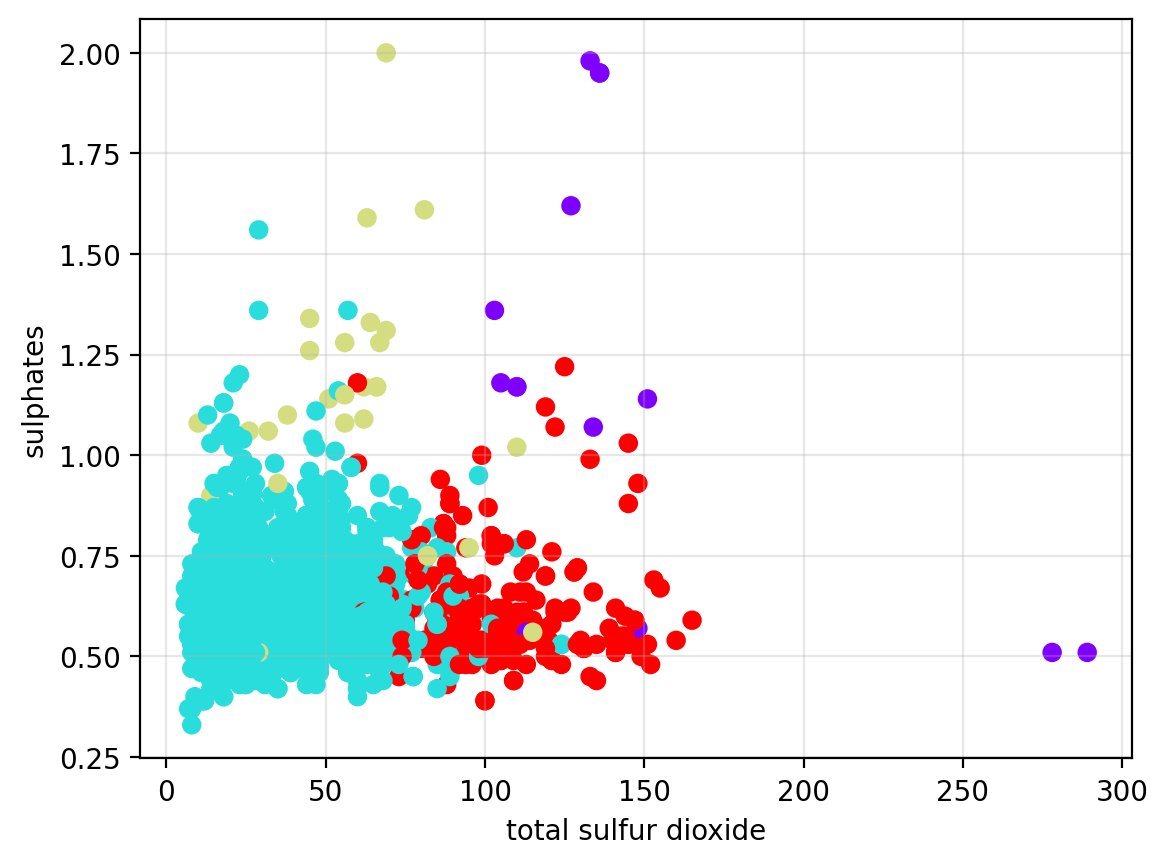
\includegraphics[width=0.67\textwidth]{images2/EM/wines/ExpectationMaximization_Wines_xtotalsulfurdioxide_ysulphates.png}
    \caption{Wizualizacja centrów dla zbioru B przy pomocy EM}
    \label{fig:em_b_2}
\end{figure}

\subsubsection*{Zbiór C}

\begin{table}[H]
    \centering
    \begin{tabular}{|l|l|l|l|}
    \hline
    \textbf{Typ kowariancji} & \textbf{Silhouette} & \textbf{Calinski-Harabasz} & \textbf{Davies-Bouldin} \\ \hline
    full                     & 0.014               & 359.952                    & 5.903                   \\ \hline
    tied                     & 0.194               & 1258.45                    & 1.742                   \\ \hline
    diag                     & -0.064              & 440.984                    & 4.07                    \\ \hline
    spherical                & 0.204               & 1427.614                   & 1.499                   \\ \hline
    \end{tabular}
    \caption{Wartości metryk dla różnych typów macierzy kowariancji algorytmu EM dla zbioru C}
    \label{tab:em_c_cov}
\end{table}

\begin{table}[H]
    \centering
    \begin{tabular}{|l|l|l|l|}
    \hline
    \textbf{Iteracja} & \textbf{Silhouette} & \textbf{Calinski-Harabasz} & \textbf{Davies-Bouldin} \\ \hline
    20                & 0.015               & 400.416                    & 3.93                    \\ \hline
    40                & -0.082              & 442.734                    & 3.262                   \\ \hline
    60                & -0.038              & 278.84                     & 4.683                   \\ \hline
    80                & 0.014               & 361.875                    & 5.897                   \\ \hline
    100               & -0.082              & 443.708                    & 3.259                   \\ \hline
    120               & -0.079              & 446.098                    & 3.306                   \\ \hline
    140               & 0.014               & 359.952                    & 5.903                   \\ \hline
    160               & -0.033              & 443.15                     & 5.37                    \\ \hline
    180               & -0.079              & 350.615                    & 4.564                   \\ \hline
    200               & -0.033              & 443.15                     & 5.37                    \\ \hline
    \end{tabular}
    \caption{Wartości metryk dla różnej maksymalnej liczby iteracji algorytmu EM dla zbioru C}
    \label{tab:em_c_iter}
\end{table}

Z tabel \ref{tab:em_c_cov} oraz \ref{tab:em_c_iter} wywnioskować można, że najlepszą konfiguracją jest \textit{spherical} oraz 100 iteracji.

\begin{figure}[H]
    \centering
    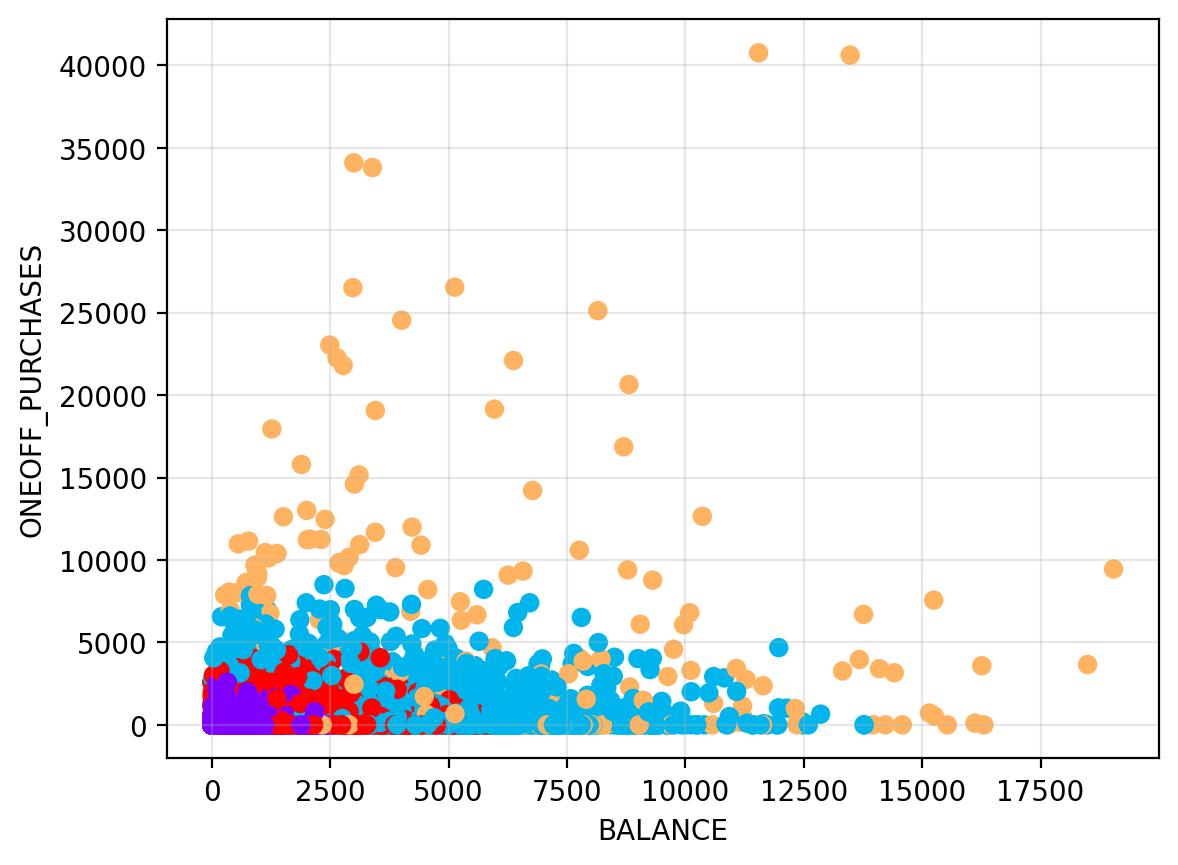
\includegraphics[width=0.67\textwidth]{images2/EM/cc/ExpectationMaximization_CC_xBALANCE_yONEOFF_PURCHASES.png}
    \caption{Wizualizacja centrów dla zbioru C przy pomocy EM}
    \label{fig:em_c_1}
\end{figure}


\begin{figure}[H]
    \centering
    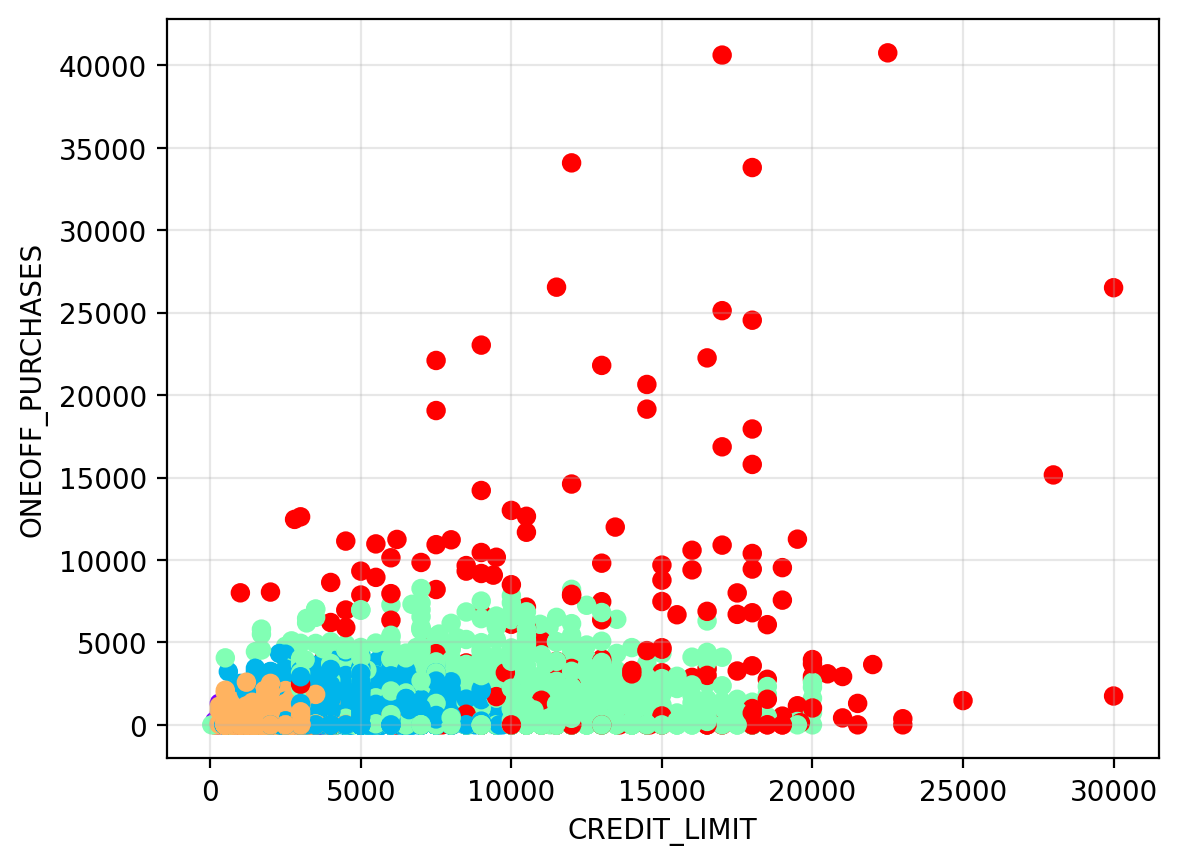
\includegraphics[width=0.67\textwidth]{images2/EM/cc/ExpectationMaximization_CC_xCREDIT_LIMIT_yONEOFF_PURCHASES.png}
    \caption{Wizualizacja centrów dla zbioru C przy pomocy EM}
    \label{fig:em_c_2}
\end{figure}


\begin{figure}[H]
    \centering
    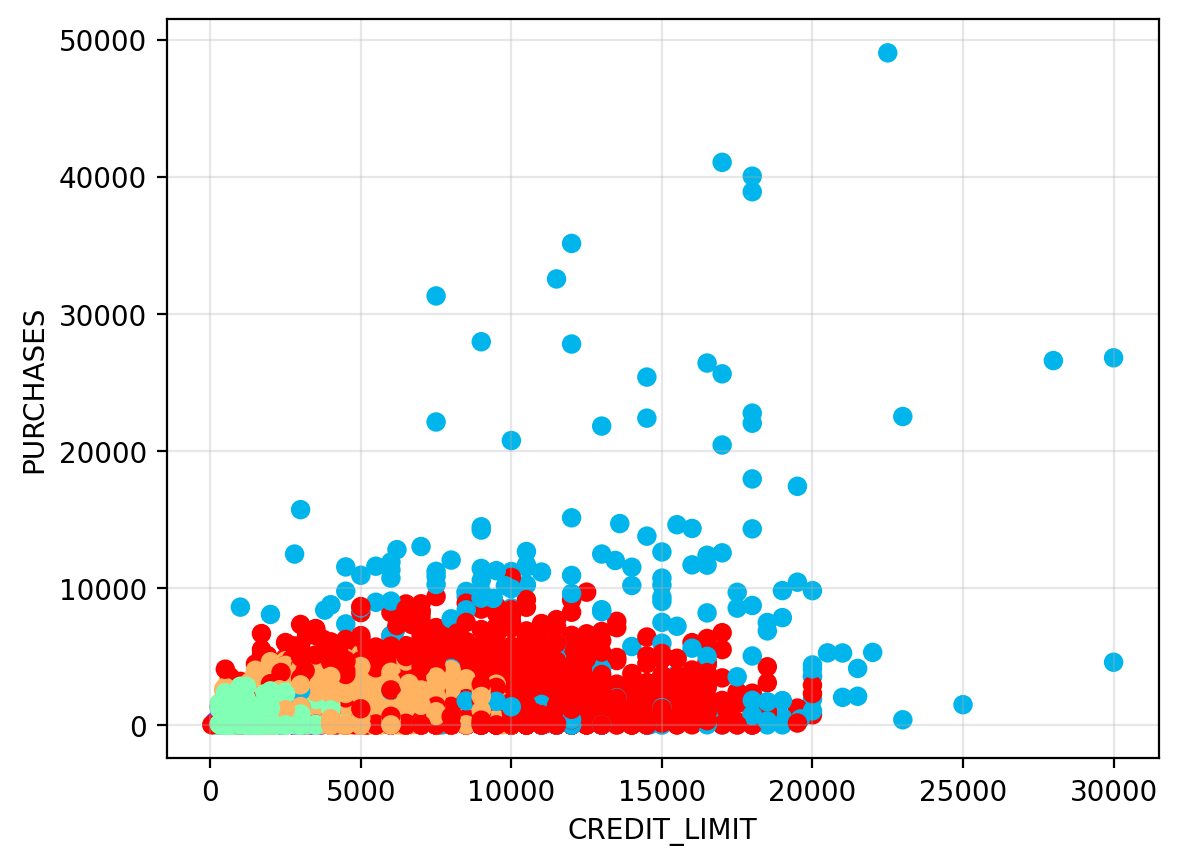
\includegraphics[width=0.67\textwidth]{images2/EM/cc/ExpectationMaximization_CC_xCREDIT_LIMIT_yPURCHASES.png}
    \caption{Wizualizacja centrów dla zbioru C przy pomocy EM}
    \label{fig:em_c_3}
\end{figure}

\subsection{Algorytm k-średnich}

Na samym początku sprawdzono wpływ powtórnego losowania centrów na uzyskane wyniki. Następnie porównano liczbę maksymalnych iteracji, po czym sprawdzono wpływ wyboru ziarna przy losowaniu centrów. Ziarna zostały wybrane zgodnie z \cite{KmeansSeeds}.

Standardowa konfiguracja obejmowała 10 uruchomień z losowaniem centrów, 50 maksymalnych iteracji oraz brak zmiany ziarna losowania.

\subsubsection*{Zbiór A}

\begin{table}[!hp]
    \centering
    \begin{tabular}{|c|c|c|c|}
    \hline
    \textbf{Uruchomienia} & \textbf{Silhouette} & \textbf{Calinski-Harabasz} & \textbf{Davies-Bouldin} \\ \hline
    1  & 0.3497 & 205.5867 & 0.9468 \\ \hline
    2  & 0.4204 & 253.8026 & 0.8705 \\ \hline
    5  & 0.4400 & 252.5983 & 0.8046 \\ \hline
    10 & 0.4251 & 253.8095 & 0.8532 \\ \hline
    20 & 0.4247 & 253.8266 & 0.8568 \\ \hline
    \end{tabular}
    \caption{Wartości metryk dla różnej liczby losowań początkowych centrów, dla zbioru A z wykorzystaniem algorytmu k-średnich}
    \label{tab:km_a_1}
\end{table}

\begin{table}[H]
    \centering
    \begin{tabular}{|c|c|c|c|}
    \hline
    \textbf{Maks. iteracje} & \textbf{Silhouette} & \textbf{Calinski-Harabasz} & \textbf{Davies-Bouldin} \\ \hline
    5   & 0.4400 & 252.5983 & 0.8046 \\ \hline
    10  & 0.4247 & 253.8266 & 0.8568 \\ \hline
    20  & 0.4204 & 253.8026 & 0.8705 \\ \hline
    50  & 0.4337 & 253.1832 & 0.8343 \\ \hline
    100 & 0.4337 & 253.1832 & 0.8343 \\ \hline
    \end{tabular}
    \caption{Wartości metryk dla różnej liczby maksymalnych iteracji, dla zbioru A z wykorzystaniem algorytmu k-średnich}
    \label{tab:km_a_2}
\end{table}

\begin{table}[H]
    \centering
    \begin{tabular}{|c|c|c|c|}
    \hline
    \textbf{Ziarno} & \textbf{Silhouette} & \textbf{Calinski-Harabasz} & \textbf{Davies-Bouldin} \\ \hline
    Domyślne & 0.4332 & 253.0810 & 0.8233 \\ \hline
    0        & 0.4282 & 253.8041 & 0.8456 \\ \hline
    42       & 0.4216 & 253.8315 & 0.8668 \\ \hline
    \end{tabular}
    \caption{Wartości metryk dla różnego ziarna, dla zbioru A z wykorzystaniem algorytmu k-średnich}
    \label{tab:km_a_3}
\end{table}

Uzyskane wyniki wskazują na brak większej zależności zmiany parametrów na uzyskane rezultaty wybranych metryk. Na wizualizacji \ref{tab:km_a_wis} zastosowano domyślne parametry uruchomienia.

\begin{figure}[H]
    \centering
    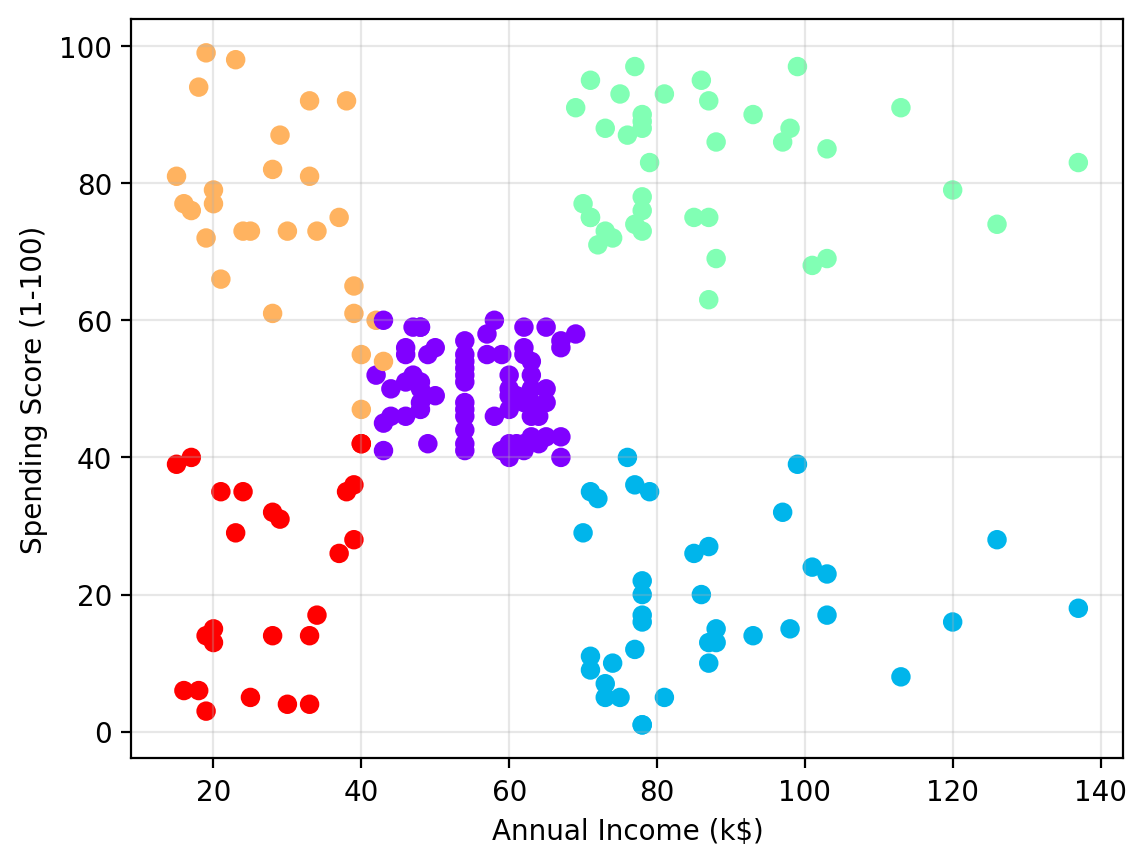
\includegraphics[width=0.67\textwidth]{images2/kmeans/Kmeans_Customer.png}
    \caption{Wizualizacja centrów dla zbioru A z wykorzystaniem algorytmu k-średnich}
    \label{tab:km_a_wis}
\end{figure}

\subsubsection*{Zbiór B}

\begin{table}[H]
    \centering
    \begin{tabular}{|c|c|c|c|}
    \hline
    \textbf{Uruchomienia} & \textbf{Silhouette} & \textbf{Calinski-Harabasz} & \textbf{Davies-Bouldin} \\ \hline
    1  & 0.4838 & 3051.5684 & 0.7150 \\ \hline
    2  & 0.4838 & 3051.5684 & 0.7150 \\ \hline
    5  & 0.4838 & 3051.5684 & 0.7150 \\ \hline
    10 & 0.4838 & 3051.5684 & 0.7150 \\ \hline
    20 & 0.4838 & 3051.5684 & 0.7150 \\ \hline
    \end{tabular}
    \caption{Wartości metryk dla różnej liczby losowań początkowych centrów, dla zbioru B z wykorzystaniem algorytmu k-średnich}
    \label{tab:km_b_1}
\end{table}

\begin{table}[H]
    \centering
    \begin{tabular}{|c|c|c|c|}
    \hline
    \textbf{Maks. iteracje} & \textbf{Silhouette} & \textbf{Calinski-Harabasz} & \textbf{Davies-Bouldin} \\ \hline
    5   & 0.4884 & 3050.9843 & 0.7109 \\ \hline
    10  & 0.4833 & 3051.0148 & 0.7147 \\ \hline
    20  & 0.4838 & 3051.5684 & 0.7150 \\ \hline
    50  & 0.4838 & 3051.5684 & 0.7150 \\ \hline
    100 & 0.4838 & 3051.5684 & 0.7150 \\ \hline
    \end{tabular}
    \caption{Wartości metryk dla różnej liczby maksymalnych iteracji, dla zbioru B z wykorzystaniem algorytmu k-średnich}
    \label{tab:km_b_2}
\end{table}

\begin{table}[H]
    \centering
    \begin{tabular}{|c|c|c|c|}
    \hline
    \textbf{Ziarno} & \textbf{Silhouette} & \textbf{Calinski-Harabasz} & \textbf{Davies-Bouldin} \\ \hline
    Domyślne & 0.4845 & 3051.9139 & 0.7146 \\ \hline
    0        & 0.4838 & 3051.5684 & 0.7150 \\ \hline
    42       & 0.4838 & 3051.5684 & 0.7150 \\ \hline
    \end{tabular}
    \caption{Wartości metryk dla różnego ziarna, dla zbioru B z wykorzystaniem algorytmu k-średnich}
    \label{tab:km_b_3}
\end{table}

Uzyskane wyniki wskazują na brak większej zależności zmiany parametrów na uzyskane rezultaty wybranych metryk. Na wizualizacjach \ref{tab:km_b_wis_1} oraz \ref{tab:km_b_wis_2} zastosowano domyślne parametry uruchomienia.

\begin{figure}[H]
    \centering
    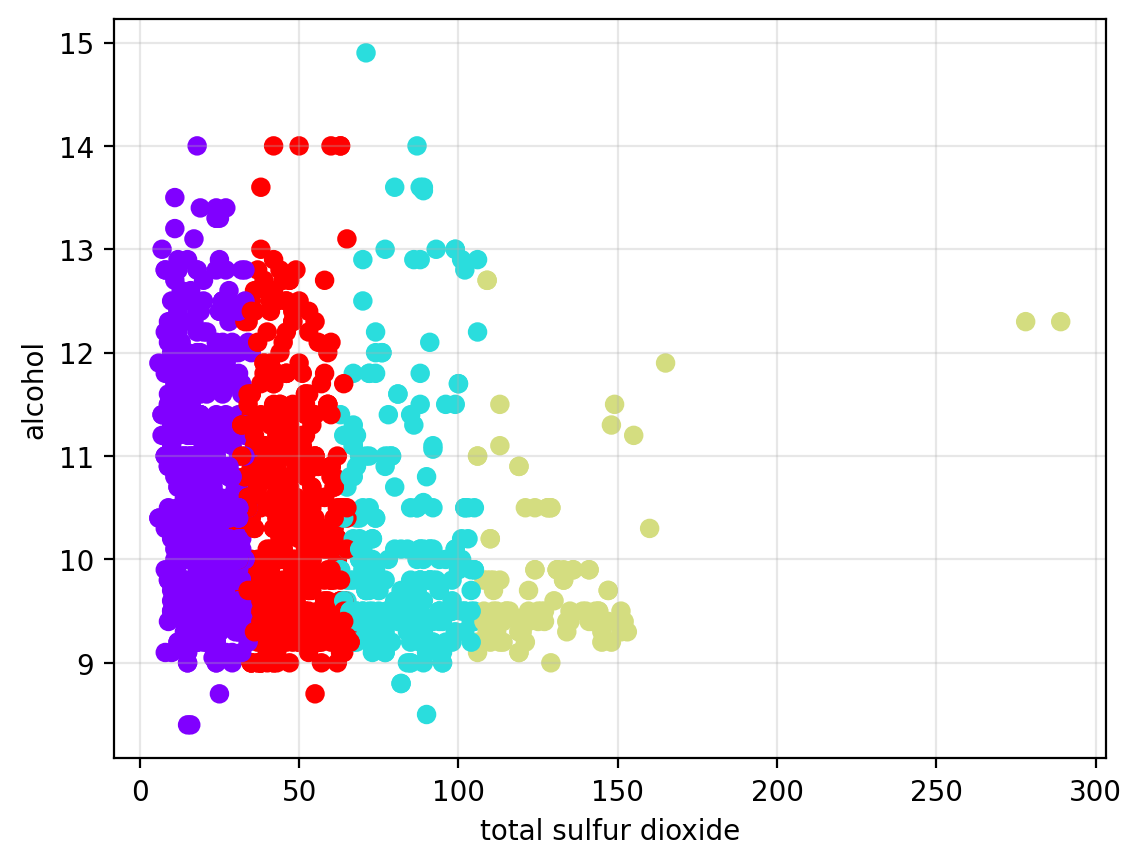
\includegraphics[width=0.67\textwidth]{images2/kmeans/Kmeans_Wines_1.png}
    \caption{Pierwsza wizualizacja centrów dla zbioru B z wykorzystaniem algorytmu k-średnich}
    \label{tab:km_b_wis_1}
\end{figure}

\begin{figure}[H]
    \centering
    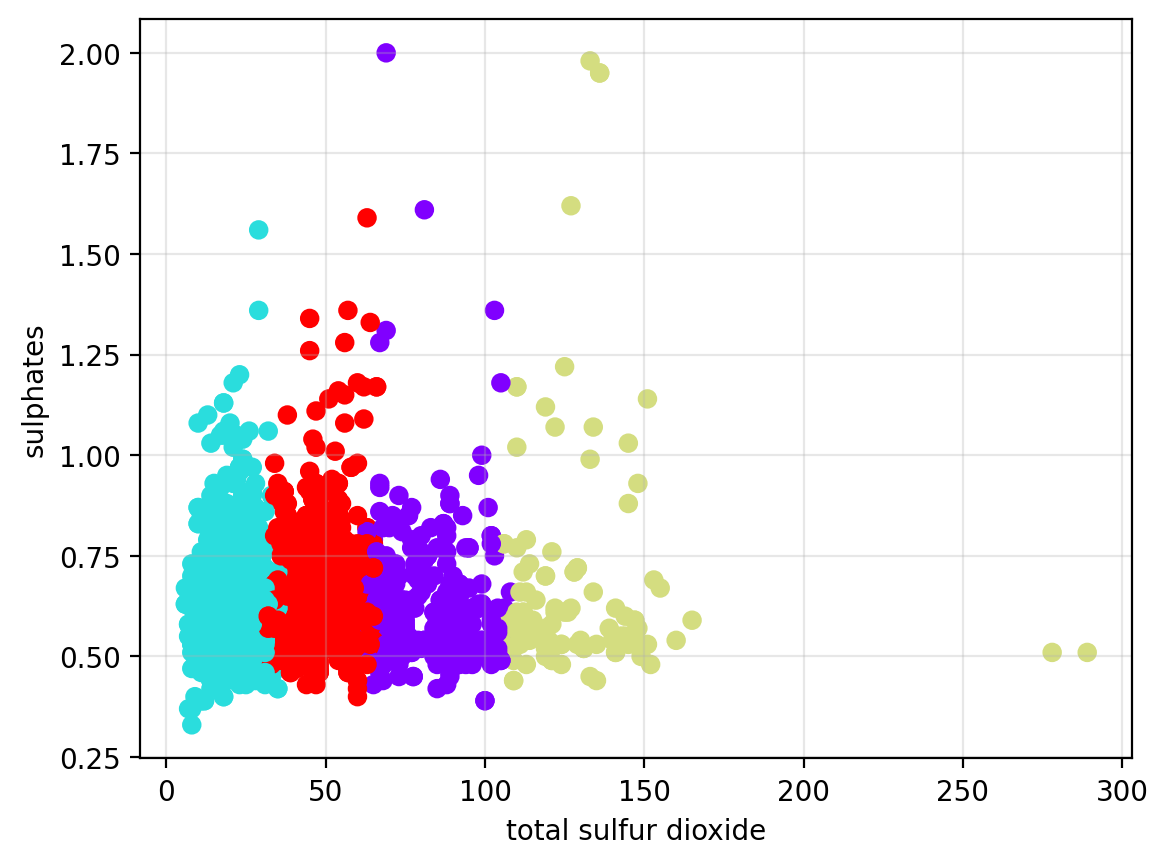
\includegraphics[width=0.67\textwidth]{images2/kmeans/Kmeans_Wines_2.png}
    \caption{Druga wizualizacja centrów dla zbioru B z wykorzystaniem algorytmu k-średnich}
    \label{tab:km_b_wis_2}
\end{figure}

\subsubsection*{Zbiór C}

\begin{table}[H]
    \centering
    \begin{tabular}{|c|c|c|c|}
    \hline
    \textbf{Uruchomienia} & \textbf{Silhouette} & \textbf{Calinski-Harabasz} & \textbf{Davies-Bouldin} \\ \hline
    1  & 0.3808 & 2549.0832 & 1.2981 \\ \hline
    2  & 0.3808 & 2549.0832 & 1.2981 \\ \hline
    5  & 0.3808 & 2549.0832 & 1.2981 \\ \hline
    10 & 0.3820 & 2549.3077 & 1.2934 \\ \hline
    20 & 0.3819 & 2549.3082 & 1.2941 \\ \hline
    \end{tabular}
    \caption{Wartości metryk dla różnej liczby losowań początkowych centrów, dla zbioru C z wykorzystaniem algorytmu k-średnich}
    \label{tab:km_c_1}
\end{table}

\begin{table}[H]
    \centering
    \begin{tabular}{|c|c|c|c|}
    \hline
    \textbf{Maks. iteracje} & \textbf{Silhouette} & \textbf{Calinski-Harabasz} & \textbf{Davies-Bouldin} \\ \hline
    5   & 0.3701 & 2540.3679 & 1.3224 \\ \hline
    10  & 0.3748 & 2542.0966 & 1.3187 \\ \hline
    20  & 0.3820 & 2549.3077 & 1.2934 \\ \hline
    50  & 0.3808 & 2549.0832 & 1.2981 \\ \hline
    100 & 0.3808 & 2549.0832 & 1.2981 \\ \hline
    \end{tabular}
    \caption{Wartości metryk dla różnej liczby maksymalnych iteracji, dla zbioru C z wykorzystaniem algorytmu k-średnich}
    \label{tab:km_c_2}
\end{table}

\begin{table}[H]
    \centering
    \begin{tabular}{|c|c|c|c|}
    \hline
    \textbf{Ziarno} & \textbf{Silhouette} & \textbf{Calinski-Harabasz} & \textbf{Davies-Bouldin} \\ \hline
    Domyślne & 0.3820 & 2549.3077 & 1.2934 \\ \hline
    0        & 0.3808 & 2549.0832 & 1.2981 \\ \hline
    42       & 0.3820 & 2549.3077 & 1.2934 \\ \hline
    \end{tabular}
    \caption{Wartości metryk dla różnego ziarna, dla zbioru C z wykorzystaniem algorytmu k-średnich}
    \label{tab:km_c_3}
\end{table}

Uzyskane wyniki wskazują na brak większej zależności zmiany parametrów na uzyskane rezultaty wybranych metryk. Na wizualizacjach \ref{tab:km_c_wis_1}, \ref{tab:km_c_wis_2} i \ref{tab:km_c_wis_3} zastosowano domyślne parametry uruchomienia.

\begin{figure}[H]
    \centering
    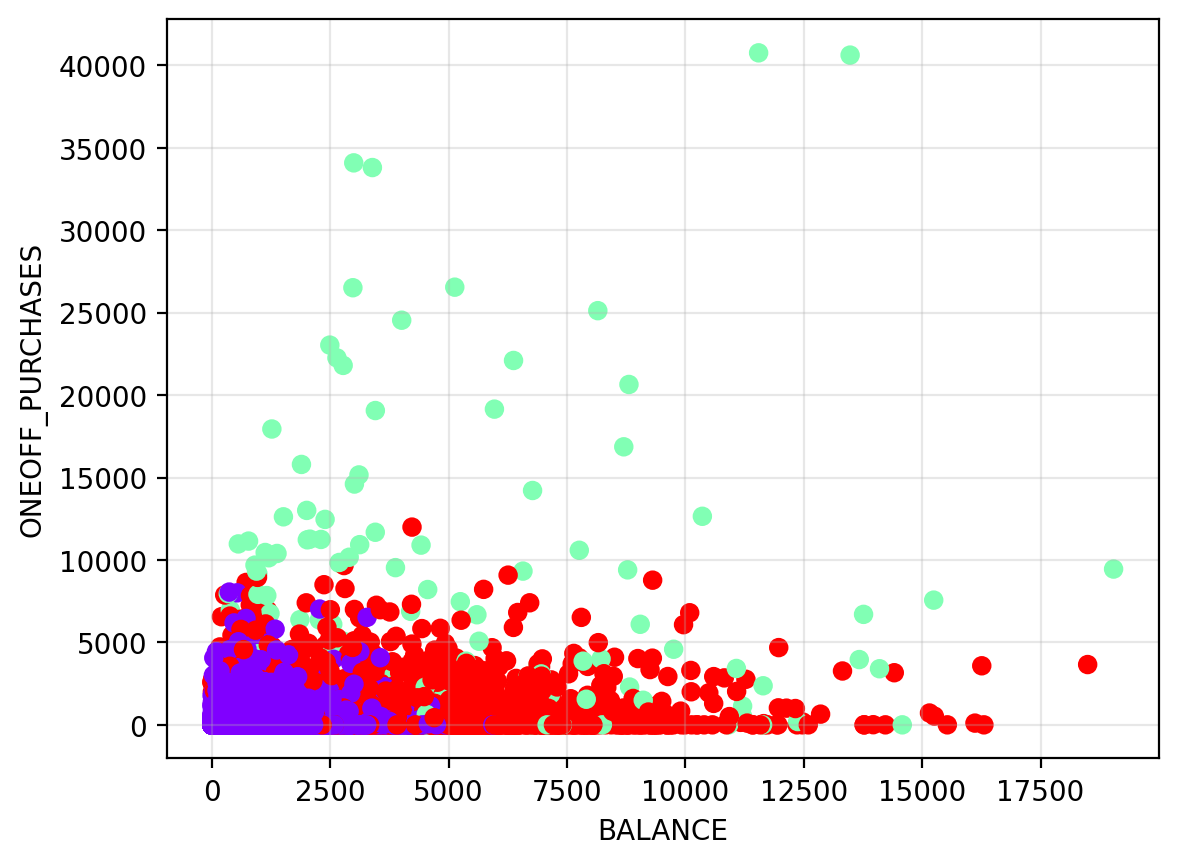
\includegraphics[width=0.67\textwidth]{images2/kmeans/Kmeans_CC_1.png}
    \caption{Pierwsza wizualizacja centrów dla zbioru C z wykorzystaniem algorytmu k-średnich}
    \label{tab:km_c_wis_1}
\end{figure}

\begin{figure}[H]
    \centering
    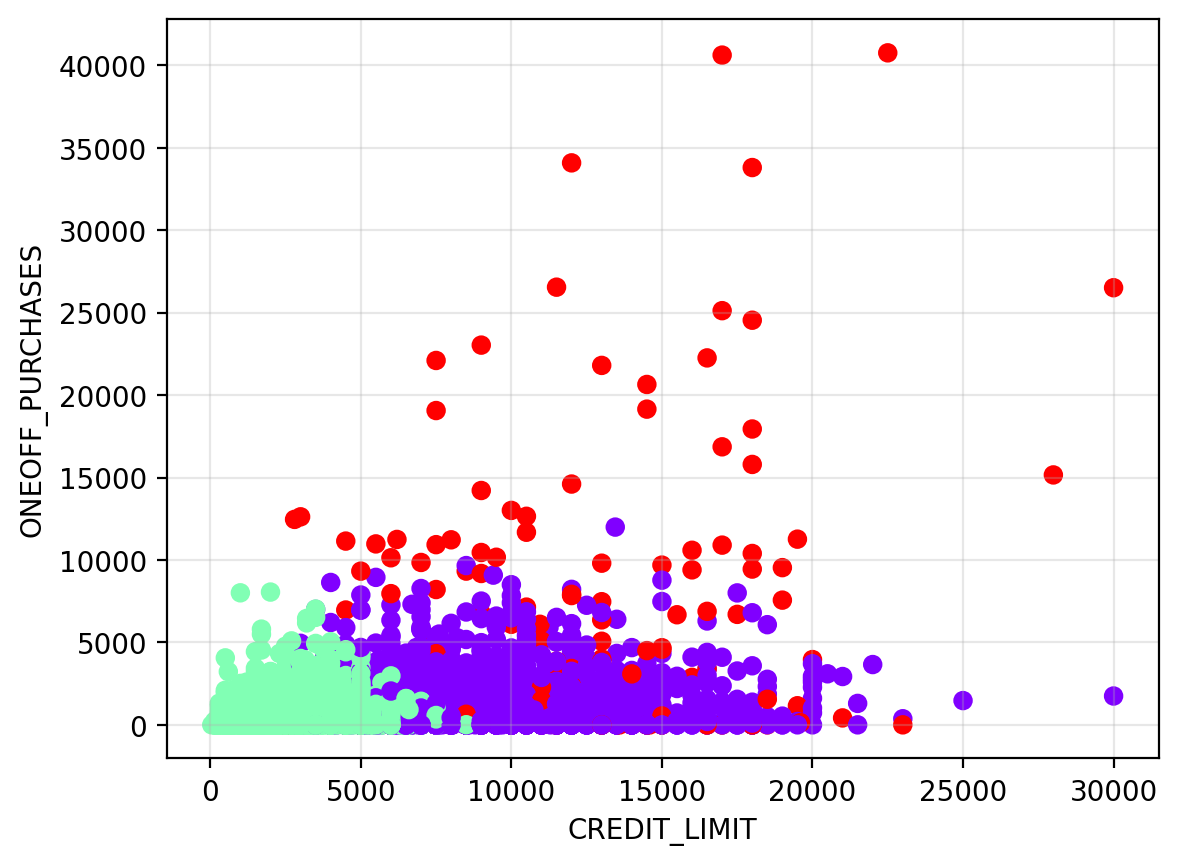
\includegraphics[width=0.67\textwidth]{images2/kmeans/Kmeans_CC_2.png}
    \caption{Druga wizualizacja centrów dla zbioru C z wykorzystaniem algorytmu k-średnich}
    \label{tab:km_c_wis_2}
\end{figure}

\begin{figure}[H]
    \centering
    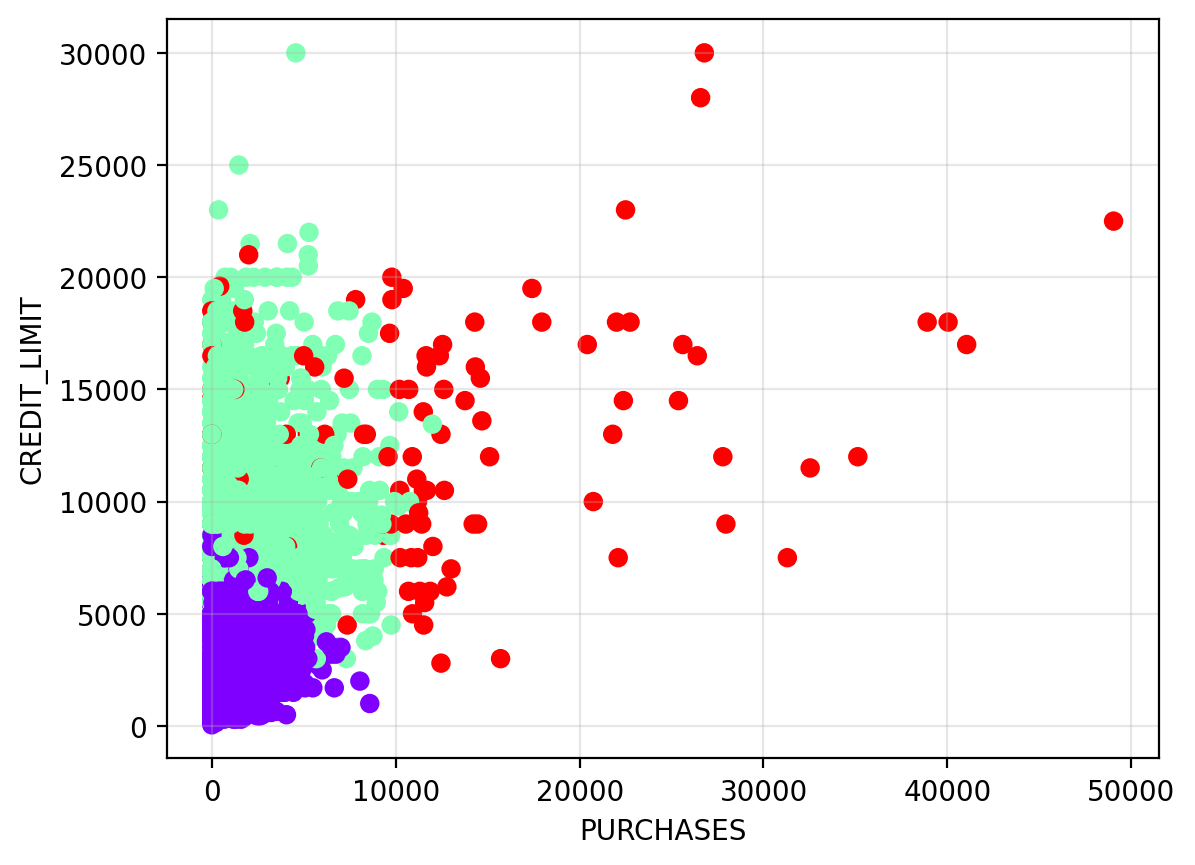
\includegraphics[width=0.67\textwidth]{images2/kmeans/Kmeans_CC_3.png}
    \caption{Trzecia wizualizacja centrów dla zbioru C z wykorzystaniem algorytmu k-średnich}
    \label{tab:km_c_wis_3}
\end{figure}

\subsection{Algorytm hierarchiczne aglomeracyjny}

    \subsubsection*{Zbiór A}
        \begin{table}[H]
            \centering
            \begin{tabular}{|l|l|l|l|}
            \hline
            \textbf{Konfiguracja} & \textbf{Silhouette} & \textbf{Calinski-Harabasz} & \textbf{Davies-Bouldin} \\ \hline
            single euclidean         & 0.212               & 94.893                     & 0.693                   \\ \hline
            single manhattan         & 0.188               & 17.934                     & 0.661                   \\ \hline
            average euclidean        & 0.443               & 243.445                    & 0.741                   \\ \hline
            average manhattan        & 0.443               & 243.445                    & 0.741                   \\ \hline
            \end{tabular}
            \caption{Wartości metryk dla różnych konfiguracji algorytmu aglomeracyjnego dla zbioru A}
            \label{tab:agg_a}
        \end{table}
        
        Na podstawie tabeli \ref{tab:agg_a} wywnioskowano, że najlepszą konfiguracją jest metryka euklidesowa i połączenia średnie. Wykorzystaną ją do wizualizacji danych na rysunku \ref{tab:agg_a_vis}
        
        \begin{figure}[H] % python main.py -a3 -d1 -p average euclidean -x3 -y4
            \centering
            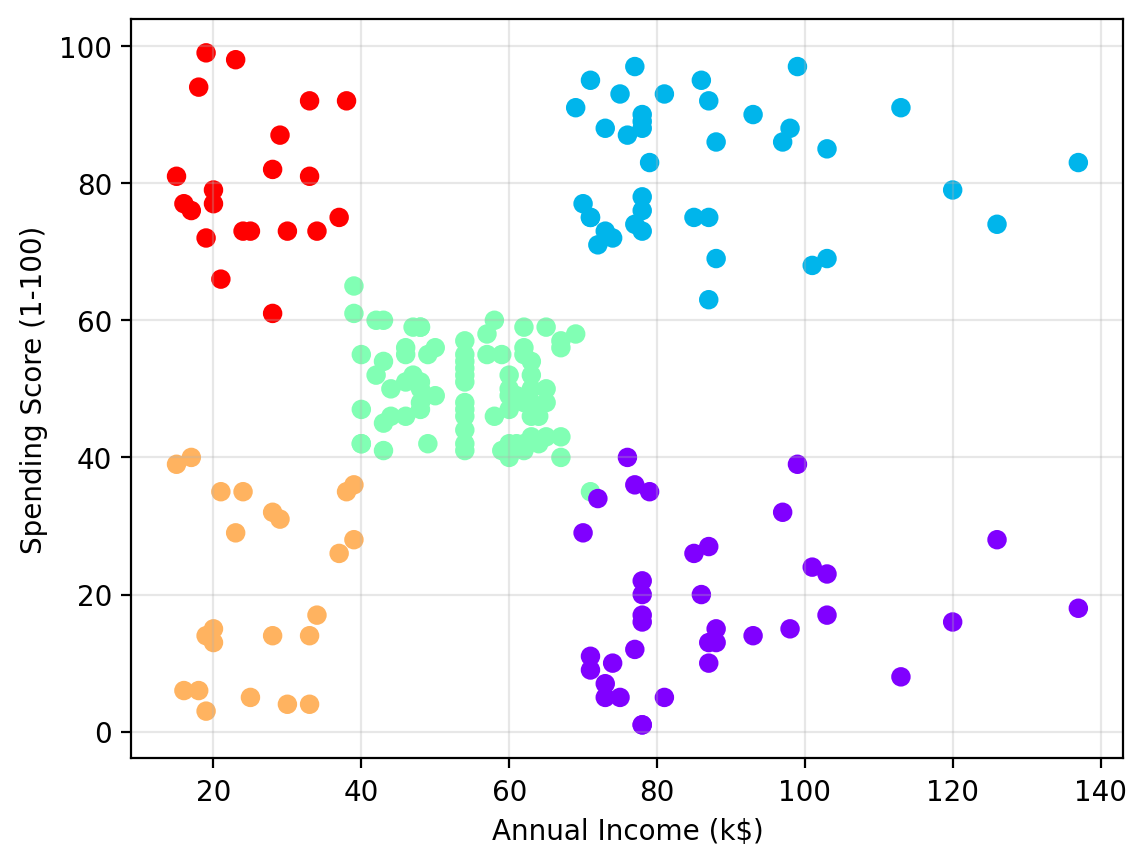
\includegraphics[width=0.67\textwidth]{images2/agglo/d1.png}
            \caption{Wizualizacja centrów dla zbioru A z wykorzystaniem algorytmu aglomeracyjnego}
            \label{tab:agg_a_vis}
        \end{figure}
    
    \subsubsection*{Zbiór B}
        \begin{table}[H]
            \centering
            \begin{tabular}{|l|l|l|l|}
            \hline
            \textbf{Konfiguracja} & \textbf{Silhouette} & \textbf{Calinski-Harabasz} & \textbf{Davies-Bouldin}    \\ \hline
            single euclidean         & 0.405               & 36.180                     & 0.298                   \\ \hline
            single manhattan         & 0.405               & 36.180                     & 0.298                   \\ \hline
            average euclidean        & 0.534               & 815.003                    & 0.604                   \\ \hline
            average manhattan        & 0.573               & 753.161                    & 0.477                   \\ \hline
            \end{tabular}
            \caption{Wartości metryk dla różnych konfiguracji algorytmu aglomeracyjnego dla zbioru B}
            \label{tab:agg_b}
        \end{table}
        
        Na podstawie tabeli \ref{tab:agg_b} widać, że ponownie najlepszą konfiguracją okazało się zestawienie metryki euklidesowej z połączeniami średnimi. Na jej podstawie wygenerowano wykresy \ref{tab:agg_b_vis1} i \ref{tab:agg_b_vis2}.
        
        \begin{figure}[H] % python main.py -a3 -d2 -p average euclidean -x6 -y10
            \centering
            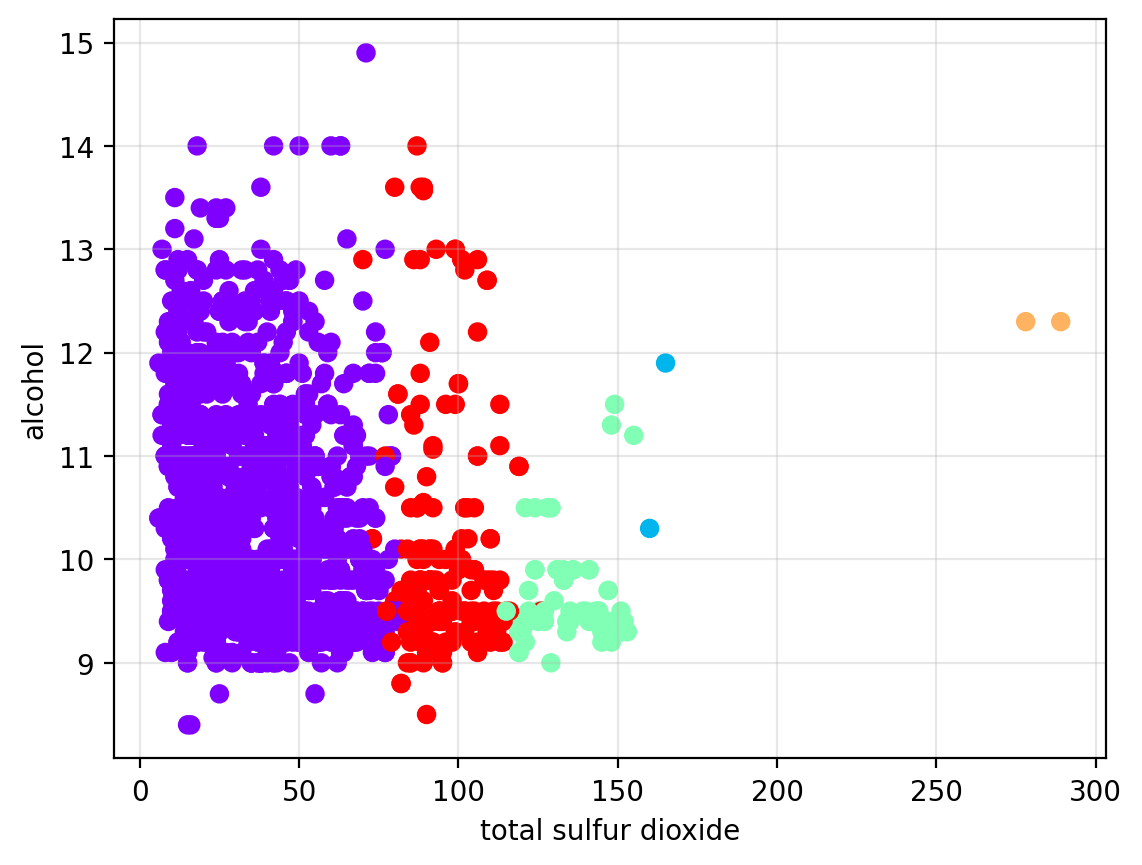
\includegraphics[width=0.67\textwidth]{images2/agglo/d2_alco.png}
            \caption{Wizualizacja centrów dla zbioru B z wykorzystaniem algorytmu aglomeracyjnego}
            \label{tab:agg_b_vis1}
        \end{figure}
        
        \begin{figure}[H] % python main.py -a3 -d2 -p average euclidean -x6 -y9
            \centering
            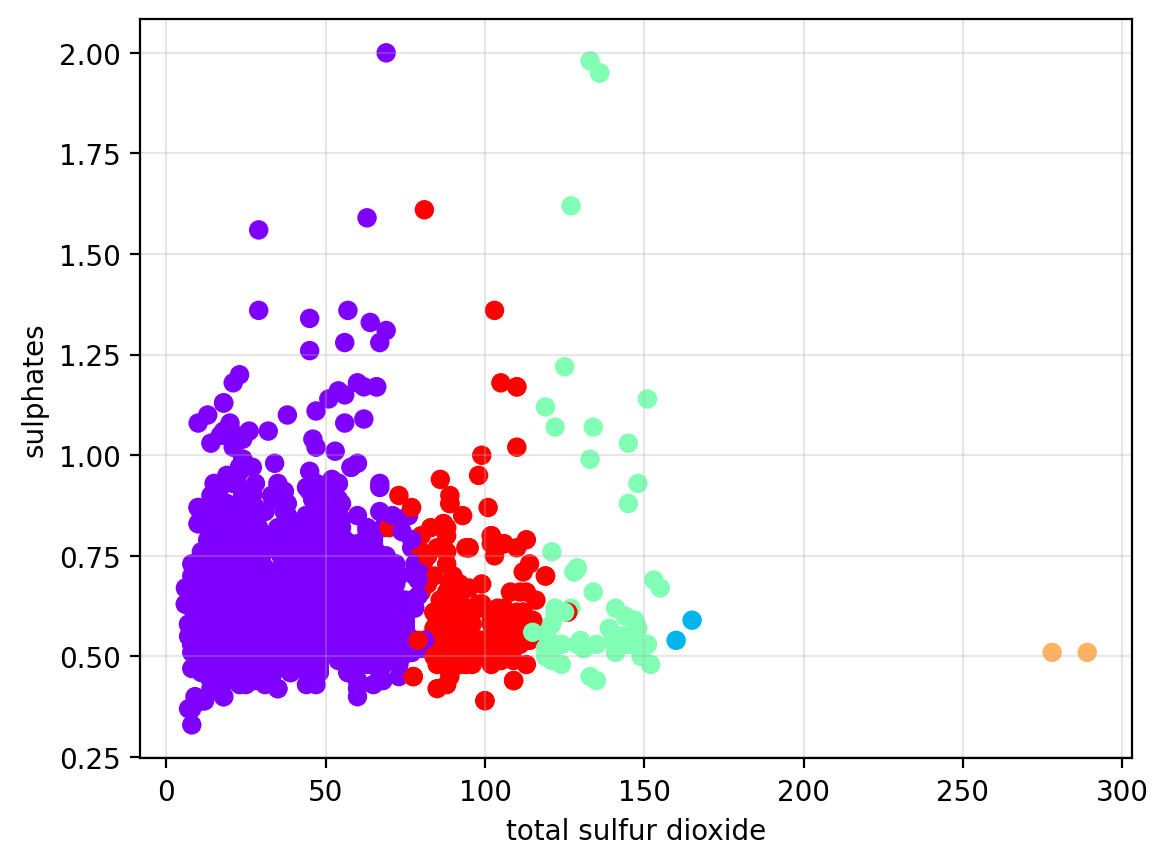
\includegraphics[width=0.67\textwidth]{images2/agglo/d2_sulf.png}
            \caption{Wizualizacja centrów dla zbioru B z wykorzystaniem algorytmu aglomeracyjnego}
            \label{tab:agg_b_vis2}
        \end{figure}
    
    \subsubsection*{Zbiór C}
        Badania dla zbioru C były niemożliwe do przeprowadzenia dla niniejszej metody klasteryzacji, ponieważ program potrzebował zbyt dużej ilości pamięci.

\subsection{Metoda gęstościowa DBSCAN}
Na początku sprawdzono jak zmiana parametru \textit{eps} wpłynęła na uzyskane wyniki. \textit{Eps} to maksymalny dystans między dwoma próbkami aby jedna została zakwalifikowana jako sąsiad tej drugiej. \\
Następnie dla ustalonego parametru sprawdzono wpływ parametru \textit{min\_samples} na wyniki. \textit{Min\_samples} to liczba próbek w sąsiedztwie dla punktu aby uznać ją za punkt rdzenny (ang. core point).
Ostatnim krokiem była wizualizacja danych dla zwycięskich parametrów. 
%%%%%%%%%%%%%
% ZBIÓR A
%%%%%%%%%%%%%
\subsubsection*{Zbiór A}

\begin{table}[H]
\centering
\begin{tabular}{|c|c|c|c|c|}
\hline
\textbf{eps} & \textbf{Silhouette} & \textbf{Calinski-Harabasz} & \textbf{Davies-Bouldin} & \textbf{Klastry} \\ \hline
8 & -0.2762 & 0.1294 & 5.9948 & 1 \\ \hline
9 & -0.3041 & 1.8672 & 3.3082 & 3 \\ \hline
10 & -0.2023 & 5.5955 & 2.7207 & 10 \\ \hline
11 & -0.1596 & 8.0735 & 2.8691 & 9 \\ \hline
12 & -0.0988 & 12.0774 & 2.1626 & 8 \\ \hline
13 & 0.0312 & 27.5645 & 2.0105 & 4 \\ \hline
14 & 0.0423 & 27.5407 & 1.5976 & 4 \\ \hline
15 & 0.1229 & 36.3278 & 1.6726 & 4 \\ \hline
16 & 0.0977 & 37.3811 & 1.5397 & 5 \\ \hline
17 & 0.3386 & 75.8489 & 1.6961 & 3 \\ \hline
18 & 0.3727 & 83.3958 & 2.0948 & 3 \\ \hline
19 & 0.2236 & 32.6268 & 2.6009 & 2 \\ \hline
20 & 0.2159 & 30.0229 & 3.2471 & 2 \\ \hline
\end{tabular}
\caption{Wartości metryk dla różnej wartości parametru \textit{eps}}
\label{tab:dbscan1}
\end{table}

Uzyskane wyniki pokazują najlepsze wyniki dla \textit{eps} równego 17.

\begin{table}[H]
\centering
\begin{tabular}{|c|c|c|c|c|}
\hline
\textbf{min\_samples} & \textbf{Silhouette} & \textbf{Calinski-Harabasz} & \textbf{Davies-Bouldin} & \textbf{Klastry} \\ \hline
1 & -0.0547 & 49.319 & 0.903 & 9 \\ \hline
2 & 0.2044 & 52.1406 & 2.474 & 7 \\ \hline
3 & 0.2186 & 59.2279 & 2.3552 & 6 \\ \hline
4 & 0.2652 & 58.1151 & 2.1279 & 4 \\ \hline
5 & 0.3386 & 75.8489 & 1.6961 & 3 \\ \hline
6 & 0.118 & 40.9146 & 1.5171 & 5 \\ \hline
7 & 0.1866 & 44.0961 & 1.747 & 5 \\ \hline
8 & 0.1806 & 37.6648 & 2.3174 & 4 \\ \hline
9 & 0.0745 & 26.6449 & 2.0137 & 4 \\ \hline
10 & -0.0076 & 21.2975 & 2.0046 & 4 \\ \hline
\end{tabular}
\caption{Wartości metryk dla różnej liczby \textit{min\_samples}}
\label{tab:dbscan11}
\end{table}

Uzyskane wyniki pokazują najlepsze wyniki dla \textit{min\_samples} równego 5.

\begin{figure}[H]
    \centering
    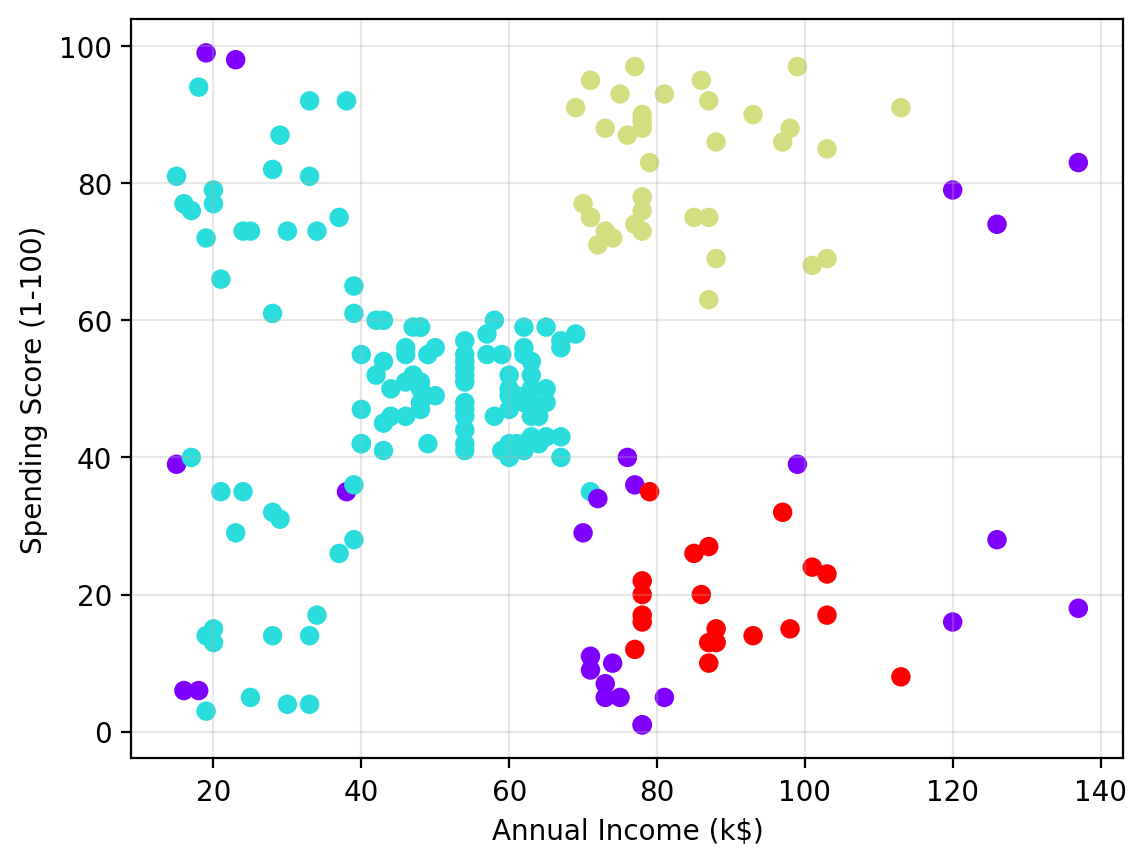
\includegraphics[width=0.67\textwidth]{images2/dbscan/d1.png}
    \caption{Wizualizacja wyliczonych centrów dla zbioru A przy pomocy DBSCAN}
    \label{fig:em_a_12}
\end{figure}

Wizualizacja dla zwycięskich wartości: \textit{eps} = 17, \textit{min\_samples} = 5.

%%%%%%%%%%%%%
% ZBIÓR B
%%%%%%%%%%%%%
\subsubsection*{Zbiór B}

\begin{table}[H]
\centering
\begin{tabular}{|c|c|c|c|c|}
\hline
\textbf{eps} & \textbf{Silhouette} & \textbf{Calinski-Harabasz} & \textbf{Davies-Bouldin} & \textbf{Klastry} \\ \hline
5 & 0.2817 & 97.6543 & 3.7493 & 6 \\ \hline
6 & 0.2803 & 96.1985 & 1.0813 & 4 \\ \hline
7 & 0.2761 & 82.1759 & 1.1353 & 2 \\ \hline
8 & 0.5727 & 151.1773 & 0.8096 & 1 \\ \hline
9 & 0.5842 & 142.9341 & 0.8203 & 1 \\ \hline
10 & 0.628 & 133.8224 & 0.7671 & 1 \\ \hline
11 & 0.6392 & 150.4493 & 0.6626 & 1 \\ \hline
12 & 0.6682 & 139.4771 & 0.6457 & 1 \\ \hline
13 & 0.6897 & 106.2034 & 0.7371 & 1 \\ \hline
14 & 0.7136 & 107.8022 & 0.6816 & 1 \\ \hline
15 & 0.7136 & 107.8022 & 0.6816 & 1 \\ \hline
16 & 0.7136 & 107.8022 & 0.6816 & 1 \\ \hline
17 & 0.7943 & 105.602 & 0.4244 & 1 \\ \hline
18 & 0.7943 & 105.602 & 0.4244 & 1 \\ \hline
19 & 0.7943 & 105.602 & 0.4244 & 1 \\ \hline
20 & 0.7943 & 105.602 & 0.4244 & 1 \\ \hline

\end{tabular}
\caption{Wartości metryk dla różnej wartości parametru \textit{eps}}
\label{tab:dbscan21}
\end{table}

Uzyskane wyniki pokazują najlepsze wyniki dla \textit{eps} równego 17 wzwyż.

\begin{table}[H]
\centering
\begin{tabular}{|c|c|c|c|c|}
\hline
\textbf{min\_samples} & \textbf{Silhouette} & \textbf{Calinski-Harabasz} & \textbf{Davies-Bouldin} & \textbf{Klastry} \\ \hline
1 & 0.6576 & 58.0027 & 0.1897 & 3 \\ \hline
2 & 0.6576 & 58.0027 & 0.1897 & 2 \\ \hline
3 & 0.7943 & 105.602 & 0.4244 & 1 \\ \hline
4 & 0.7943 & 105.602 & 0.4244 & 1 \\ \hline
5 & 0.7943 & 105.602 & 0.4244 & 1 \\ \hline
6 & 0.7943 & 105.602 & 0.4244 & 1 \\ \hline
7 & 0.7943 & 105.602 & 0.4244 & 1 \\ \hline
8 & 0.7355 & 106.0016 & 0.647 & 1 \\ \hline
9 & 0.7355 & 106.0016 & 0.647 & 1 \\ \hline
10 & 0.7355 & 106.0016 & 0.647 & 1 \\ \hline
\end{tabular}
\caption{Wartości metryk dla różnej liczby \textit{min\_samples}}
\label{tab:dbscan2}
\end{table}

Uzyskane wyniki pokazują najlepsze wyniki dla \textit{min\_samples} równego 3 (aż do 7).

\begin{figure}[H]
    \centering
    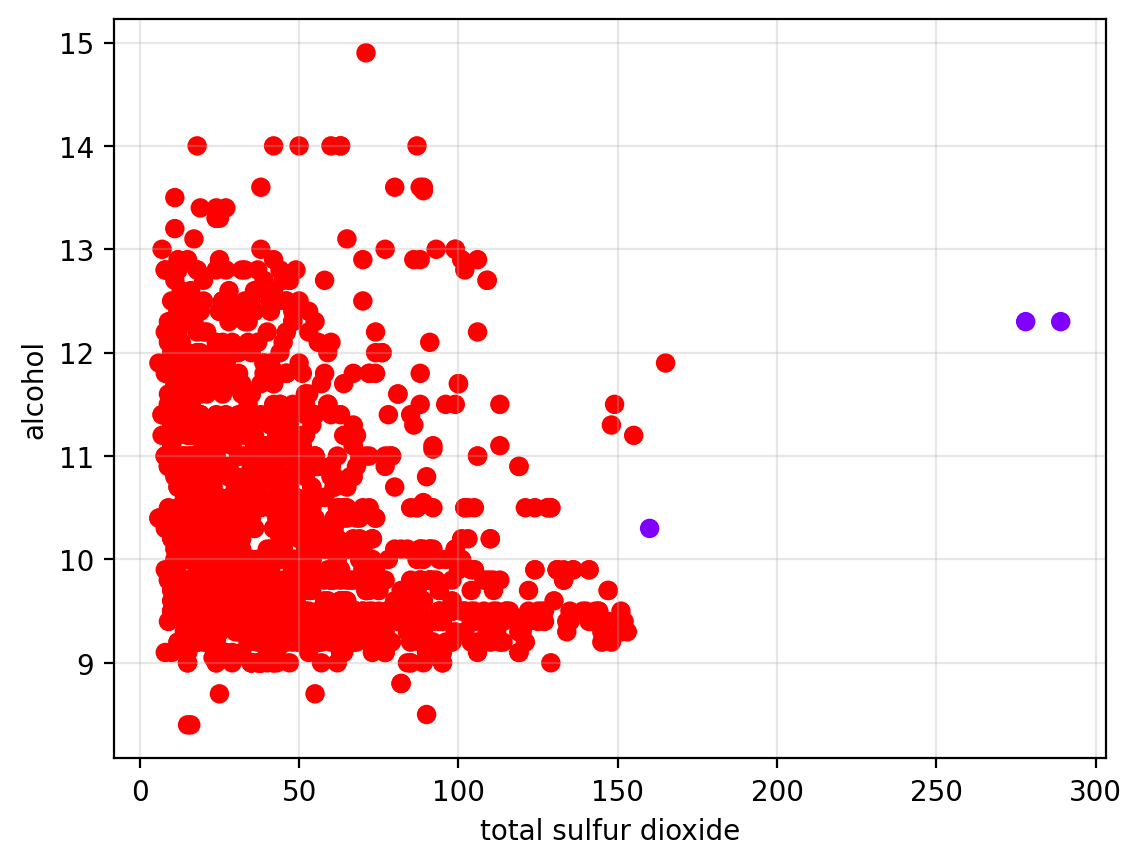
\includegraphics[width=0.67\textwidth]{images2/dbscan/d2.png}
    \caption{Wizualizacja wyliczonych centrów dla zbioru A przy pomocy DBSCAN}
    \label{fig:em_a_22}
\end{figure}

Wizualizacja dla zwycięskich wartości: \textit{eps} = 17, \textit{min\_samples} = 3.

%%%%%%%%%%%%%
% ZBIÓR C
%%%%%%%%%%%%%
\subsubsection*{Zbiór C}
Badania dla zbioru C były niemożliwe do przeprowadzenia dla niniejszej metody klasteryzacji, ponieważ program potrzebował zbyt dużej ilości pamięci.

\subsection{Algorytm optics}
Pierwszym krokiem do sprawdzenia algorytmu było ustawienie początkowych wartości dla parametrów: min-samples oraz min-cluster-size. Min-samples określa liczbę próbek leżących w sąsiedztwie punktu który bierzemy za punkt centralny natomiast min-cluster-size jest minimalna liczbą próbek w klastrze. Kolejnym korkiem było sprawdzenie otrzymanych wartości dla wybranych parametrów oraz zwizualizowanie najlepszych otrzymanych wartości.
\subsubsection*{Zbiór A}

\begin{table}[H]
    \centering
    \begin{tabular}{|c|c|c|c|}
    \hline
    \textbf{min-sample} & \textbf{Silhouette} & \textbf{Calinski-Harabasz} & \textbf{Davies-Bouldin} \\ \hline
    5   & 0.2786 & 44.3790 & 1.3174 \\ \hline
    10  & 0.2841 & 41.6443 & 1.5186 \\ \hline
    20  & 0.0455 & 18.0750 & 2.5740 \\ \hline
    30  & 0.1370 & 7.2539 & 4.1196 \\ \hline
    40 & 0.2406 & 11.6215 & 3.8548 \\ \hline
    50 & 0.0824 & 2.5170 & 6.6239 \\ \hline
    \end{tabular}
    \caption{Wartości metryk dla różnej liczby minimalnych próbek, dla zbioru A z wykorzystaniem algorytmu optics}
    \label{tab:op_a_1}
\end{table}
\begin{table}[H]
    \centering
    \begin{tabular}{|c|c|c|c|}
    \hline
    \textbf{min-cluster-size} & \textbf{Silhouette} & \textbf{Calinski-Harabasz} & \textbf{Davies-Bouldin} \\ \hline
    0.05   & -0.1135 & 13.3816 & 3.4582 \\ \hline
    0.1  & -0.0539 & 22.4077 & 2.7230 \\ \hline
    0.5  & 0.2786 & 44.3790 & 1.3174 \\ \hline
    2  & -0.1550 & 8.4379 & 1.9298 \\ \hline
    5 & -0.1793 & 8.9151 & 2.1548 \\ \hline
    10 & -0.1135 & 13.3816 & 3.4582 \\ \hline
    \end{tabular}
    \caption{Wartości metryk dla różnej liczby minimalnych próbek, dla zbioru A z wykorzystaniem algorytmu optics}
    \label{tab:op_a_2}
\end{table}
Najlepszą konfiguracją jest minimalny rozmiar klastra = 0.5 oraz minimalna liczba próbek = 5 
\begin{figure}[!htbp]
    \centering
    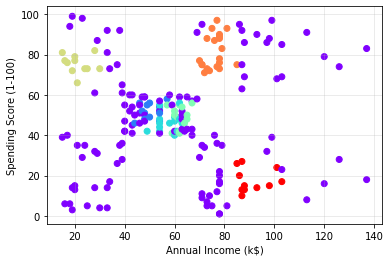
\includegraphics[width=0.67\textwidth]{images2/op/opA.png}
    \caption{Wizualizacja wyliczonych centrów dla zbioru A przy pomocy optics}
    \label{fig:op_i_3}
\end{figure}

\subsubsection*{Zbiór B}
\begin{table}[H]
    \centering
    \begin{tabular}{|c|c|c|c|}
    \hline
    \textbf{min-sample} & \textbf{Silhouette} & \textbf{Calinski-Harabasz} & \textbf{Davies-Bouldin} \\ \hline
    5   & -0.4254 & 15.0433 & 1.6694 \\ \hline
    10  & -0.6121 & 9.9393 & 2.3454 \\ \hline
    20  & -0.4769 & 22.4975 & 1.0388 \\ \hline
    30  & 0.2597 & 112.3621 & 0.7562 \\ \hline
    40 & 0.5958 & 682.6572 & 0.5330 \\ \hline
    \end{tabular}
    \caption{Wartości metryk dla różnej liczby minimalnych próbek, dla zbioru B z wykorzystaniem algorytmu optics}
    \label{tab:op_b_1}
\end{table}
\begin{table}[H]
    \centering
    \begin{tabular}{|c|c|c|c|}
    \hline
    \textbf{min-cluster-size} & \textbf{Silhouette} & \textbf{Calinski-Harabasz} & \textbf{Davies-Bouldin} \\ \hline
    0.05   & 0.5958 & 682.6572 & 0.5330 \\ \hline
    0.1  & 0.5958 & 682.6572 & 0.5330 \\ \hline
    0.5  & 0.5958 & 682.6572 & 0.5330 \\ \hline
    2  & 0.5958 & 682.6572 & 0.5330 \\ \hline
    5  & 0.5958 & 682.6572 & 0.5330 \\ \hline
    10  & 0.5958 & 682.6572 & 0.5330 \\ \hline
    20  & 0.5958 & 682.6572 & 0.5330 \\ \hline
    30  & 0.5958 & 682.6572 & 0.5330 \\ \hline
    \end{tabular}
    \caption{Wartości metryk dla różnej liczby minimalnych próbek, dla zbioru B z wykorzystaniem algorytmu optics}
    \label{tab:op_b_2}
\end{table}
Wartości metryk nie uległy zmianie pod wpływem dobierania różnych minimalnych wartości rozmiarów clastra. Metryki osiągnęły najlepsze wartości dla minimalnej liczby próbek wynoszącej 40
\begin{figure}[!htbp]
    \centering
    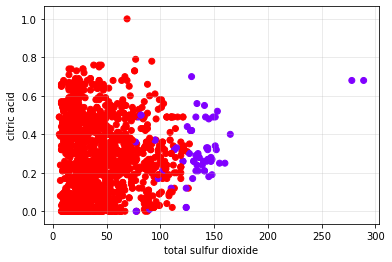
\includegraphics[width=0.67\textwidth]{images2/op/opB40.png}
    \caption{Wizualizacja wyliczonych centrów dla zbioru B przy pomocy optics}
    \label{fig:op_i_2}
\end{figure}
\subsubsection*{Zbiór C}
Badania dla zbioru C były niemożliwe do przeprowadzenia dla niniejszej metody klasteryzacji, ponieważ program potrzebował zbyt dużej ilości pamięci.
%%%%%%%%%%%%%%%%%%%%%%%%%%%%%%%%%%%%%%%%%%%% WNIOSKI

\newpage

\section{Wnioski}

\subsection*{Algorytm EM}
\begin{itemize}
    \item W związku z tym, że algorytm potrzebuje na wstępie informacji o liczbie centrów, wymagana jest wcześniejsza wiedza na temat zawartości zbioru oraz spodziewane klasy.
    \item Najlepsze konfiguracje różniły się między zbiorami danych, także ważnym elementem jest ich dobranie do każdego zbioru oddzielnie.
    \item Zwiększanie liczby iteracji powyżej pewnej wartości jest bezcelowe, ponieważ wymagana dokładność osiągana będzie zanim ustawiona liczba będzie osiągnięta.
\end{itemize}

\subsection*{Algorytm k-średnich}
\begin{itemize}
    \item W związku z tym, że algorytm potrzebuje na wstępie informacji o liczbie centrów, wymagana jest wcześniejsza wiedza na temat zawartości zbioru oraz spodziewane klasy.
    \item W przypadku wybranych zbiorów danych A, B oraz C zmiana parametrów takich jak liczba losowań centrów, maksymalne iteracje czy zmiana ziarna nie miała znacznego wpływu na uzyskane rezultaty klasyfikacji.
    \item Algorytm dąży do przypisania każdemu centrowi równej liczby elementów, co w określonych wypadkach może pogarszać wyniki.
\end{itemize}

\subsection*{Algorytm hierarchiczne aglomeracyjny}
\begin{itemize}
    \item W związku z tym, że algorytm potrzebuje na wstępie informacji o liczbie centrów, wymagana jest wcześniejsza wiedza na temat zawartości zbioru oraz spodziewane klasy.
    \item Dobrze radzi sobie przy zbiorze A, gdzie klastry są od siebie wyraźniej oddzielone niż w zbiorze B.
    \item Wrażliwy na wartości odstające.
    \item Nieoptymalny pod kątem obliczeniowym.
\end{itemize}

\subsection*{Metoda gęstościowa DBSCAN}
\begin{itemize}
    \item Algorytm przyzwoicie radzi sobie z klasteryzacją.
    \item Ze względu na specyfikacje algorytmu, aby upewnić się czy liczba klastrów jest zadowalająca, należy zastosować metryki w celu porównania wyników. Przekłada się to na różne wyniki (zależne od zastosowanej metryk) jak i na dodatkową pracę. 
\end{itemize}
\subsection*{Algorytm optics}
\begin{itemize}
    \item Algorytm optics lepiej radzi sobie z dużymi zbiorami niż algorytm DBSCAN.
    \item  Nie wymaga specjalnego dostrajania poszczególnych parametrów
\end{itemize}

%%%%%%%%%%%%%%%%%%%%%%%%%%%%%%%%%%%%%%%%%%%% BIBLIOGRAFIA

\newpage
\begin{thebibliography}{0}

    \bibitem{ClusteringQuality}
    \textsl{Prelekcja Christiana Henniga dotycząca oceny jakości klasteryzacji, \url{https://www.youtube.com/watch?v=Mf6MqIS2ql4}}

    \bibitem{KmeansSeeds}
    \textsl{Popularne wartości ziarna dla algorytmów pakietu Scikit-learn, \url{https://scikit-learn.org/stable/glossary.html\#term-random-state}}
    
\end{thebibliography}

\end{document}
